%\documentclass[12pt]{article}

\questionheader{ex:s3.7}


%%%%%%%%%%%%%%%%%%
\subsection*{\Conceptual}
%%%%%%%%%%%%%%%%%%

%%%%%%%%%%%%%%%%%%%%%%%%%%%%%%%%%%%%%%%%%
\begin{question}
Use $(\rho,\theta,\varphi)$ to denote spherical coordinates.
\begin{enumerate}[(a)]
\item
Draw $\varphi=0$.
\item
Draw $\varphi=\nicefrac{\pi}{4}$.
\item 
Draw $\varphi=\nicefrac{\pi}{2}$.
\item
Draw $\varphi=\nicefrac{3\pi}{4}$.
\item
Draw $\varphi=\pi$.
\end{enumerate}

\end{question}

%\begin{hint}
%
%\end{hint}

\begin{answer}
\begin{center}
   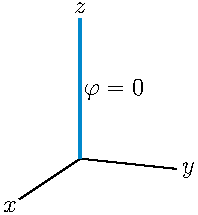
\includegraphics{fig/spherPhi0.pdf}\qquad\quad
   \raisebox{0.0\height}{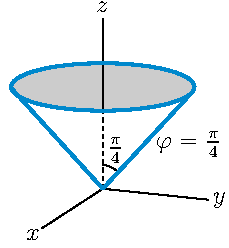
\includegraphics[scale=1.0]{fig/spherPhiUp.pdf}}
      \qquad\quad
   \raisebox{0.3\height}{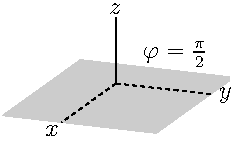
\includegraphics[scale=1.0]{fig/spherPhiFl.pdf}}
\end{center}
\begin{center}
   \raisebox{0.0\height}{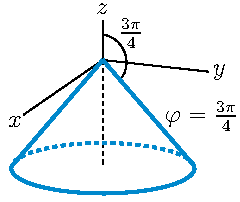
\includegraphics[scale=1.0]{fig/spherPhiDn.pdf}}
\qquad\qquad
   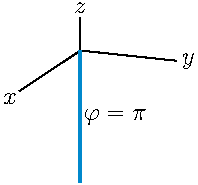
\includegraphics{fig/spherPhiPi.pdf}
\end{center}
\end{answer}

\begin{solution}
Since the spherical coordinate $\varphi(x,y,z)$ of a point $(x,y,z)$ is
the angle between the positive $z$-axis and the radius vector from 
$(0,0,0)$ to $(x,y,z)$, the sets
\begin{align*}
\Set{(x,y,z)}{\varphi(x,y,z)=0}
&=\text{the positive $z$-axis} \\
\Set{(x,y,z)}{\varphi(x,y,z)=\nicefrac{\pi}{2}}
&=\text{the $xy$-plane} \\
\Set{(x,y,z)}{\varphi(x,y,z)=\pi}
&=\text{the negative $z$-axis} 
\end{align*} 
Alternatively, $\tan\varphi(x,y,z)=\frac{z}{\sqrt{x^2+y^2}}$, so that,
for any $0<\Phi<\pi$,
\begin{align*}
\Set{(x,y,z)}{\varphi(x,y,z)=\Phi}
&=\Set{(x,y,z)}{z=\tan\Phi\sqrt{x^2+y^2}} \\
&=\text{the cone that makes the angle $\Phi$ with the positive $z$-axis} 
\end{align*} 
\begin{center}
   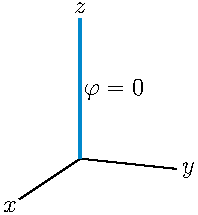
\includegraphics{fig/spherPhi0.pdf}\qquad\quad
   \raisebox{0.0\height}{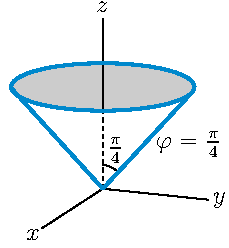
\includegraphics[scale=1.0]{fig/spherPhiUp.pdf}}
      \qquad\quad
   \raisebox{0.3\height}{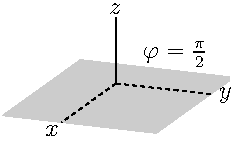
\includegraphics[scale=1.0]{fig/spherPhiFl.pdf}}
\end{center}
\begin{center}
   \raisebox{0.0\height}{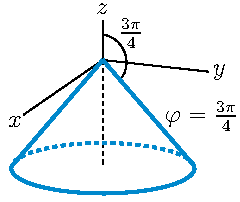
\includegraphics[scale=1.0]{fig/spherPhiDn.pdf}}
\qquad\qquad
   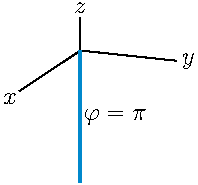
\includegraphics{fig/spherPhiPi.pdf}
\end{center}
\end{solution}


%%%%%%%%%%%%%%%%%%%%%%%%%%%%%%%%%%%%%%%%%
\begin{question}
Sketch the point with the specified spherical coordinates.
\begin{enumerate}[(a)]
\item
$\rho=0$, $\theta=0.1\pi$, $\varphi=0.7\pi$
\item
$\rho=1$, $\theta=0.3\pi$, $\varphi=0$
\item
$\rho=1$, $\theta=0$, $\varphi=\frac{\pi}{2}$
\item
$\rho=1$, $\theta=\frac{\pi}{3}$, $\varphi=\frac{\pi}{2}$
\item
$\rho=1$, $\theta=\frac{\pi}{2}$, $\varphi=\frac{\pi}{2}$
\item
$\rho=1$, $\theta=\frac{\pi}{3}$, $\varphi=\frac{\pi}{6}$
\end{enumerate}

\end{question}

%\begin{hint}
%
%\end{hint}

\begin{answer}
\begin{center}
   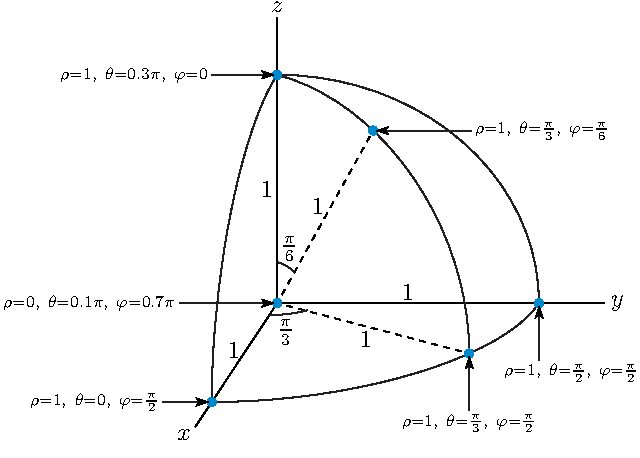
\includegraphics{fig/sphericalP1.pdf}
\end{center}
\end{answer}

\begin{solution}
The sketch is below. To help build up this sketch, it is useful to 
recall the following facts.
\begin{itemize}
\item
The spherical coordinate $\rho$ is the distance of the point from the 
origin $(0,0,0)$.
In particular if $\rho=0$, then the point is the origin (regardless of the values of $\theta$ and $\varphi$). If $\rho=1$ then the point lies on the 
sphere of radius $1$ centred on the origin.
\item
The spherical coordinate $\varphi$ is the angle between the positive $z$-axis 
and the radial line segment from the origin to $(x,y,z)$.
In particular, all points with $\varphi=0$ lie on the positive $z$--axis
(regardless of the value of $\theta$). All points with $\varphi=\frac{\pi}{2}$
lie in the $xy$-plane.
\end{itemize}
\begin{center}
   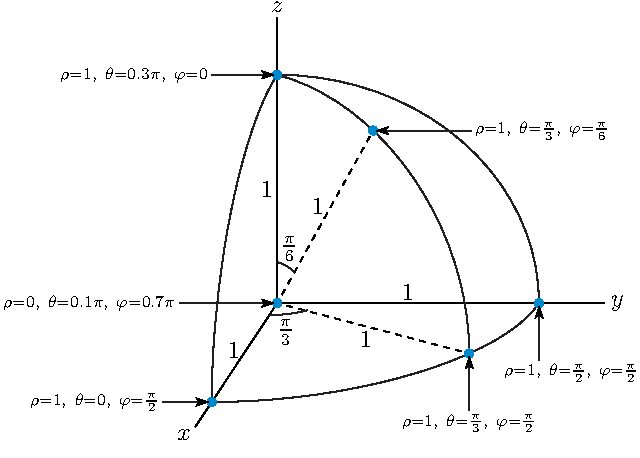
\includegraphics{fig/sphericalP1.pdf}
\end{center}
\end{solution}

%%%%%%%%%%%%%%%%%%%%%%%%%%%%%%%%%%%%%%%%%
\begin{question}
Convert from Cartesian to spherical coordinates.
\begin{enumerate}[(a)]
\item $(-2,0,0)$
\item $(0,3,0)$
\item $(0,0,-4)$
\item $\left(-\frac{1}{\sqrt{2}},\frac{1}{\sqrt{2}},\sqrt{3}\right)$
\end{enumerate}

\end{question}

%\begin{hint}
%
%\end{hint}

\begin{answer}
(a) $\rho=2$, $\theta=\pi$, $\varphi=\frac{\pi}{2}$

(b) $\rho=3$, $\theta=\frac{\pi}{2}$, $\varphi=\frac{\pi}{2}$

(c) $\rho=4$, $\theta=\text{arbitrary}$, $\varphi=\pi$

(d) $\rho=2$, $\theta=\frac{3\pi}{4}$, $\varphi=\frac{\pi}{6}$

\end{answer}

\begin{solution}
(a) The point $(-2,0,0)$
\begin{itemize}
\item 
lies in the $xy$-plane (i.e. has $z=\rho\cos\varphi=0$) and so has $\varphi=\frac{\pi}{2}$ and
\item
lies on the negative $x$-axis and so has $\theta=\pi$ and
\item
is a distance $2$ from the origin and so has $\rho=2$.
\end{itemize}

(b) The point $(0,3,0)$
\begin{itemize}
\item 
lies in the $xy$-plane (i.e. has $z=\rho\cos\varphi=0$) and so has $\varphi=\frac{\pi}{2}$ and
\item
lies on the positive $y$-axis and so has $\theta=\frac{\pi}{2}$ and
\item
is a distance $3$ from the origin and so has $\rho=3$.
\end{itemize}

(c) The point $(0,0,-4)$
\begin{itemize}
\item
lies on the negative $z$-axis and so has $\varphi=\pi$ and $\theta$ arbitrary
and
\item
is a distance $4$ from the origin and so has $\rho=4$.
\end{itemize}

(d) The point $\left(-\frac{1}{\sqrt{2}},\frac{1}{\sqrt{2}},\sqrt{3}\right)$
\begin{itemize}
\item
has $\rho=\sqrt{x^2+y^2+z^2}
       =\sqrt{\left(-\frac{1}{\sqrt{2}}\right)^2
               +\left(\frac{1}{\sqrt{2}}\right)^2
               +\left(\sqrt{3}\right)^2}=\sqrt{4}=2$
and
\item
has $\sqrt{3}=z=\rho\cos\varphi = 2\cos\varphi$ so that
$\cos\varphi = \frac{\sqrt{3}}{2}$ and $\varphi=\frac{\pi}{6}$
and
\item
has $-\frac{1}{\sqrt{2}}=x=\rho\sin\varphi\cos\theta 
= 2\big(\frac{1}{2}\big)\cos\theta$ 
so that $\cos\theta = -\frac{1}{\sqrt{2}}$. As 
$\left(-\frac{1}{\sqrt{2}},\frac{1}{\sqrt{2}}\right)$ is in the second
quadrant, we have $\frac{\pi}{2}\le\theta\le\pi$ and so 
$\theta=\frac{3\pi}{4}$.  

\end{itemize}

\end{solution}


%%%%%%%%%%%%%%%%%%%%%%%%%%%%%%%%%%%%%%%%%
\begin{question}
Convert from spherical to Cartesian coordinates.
\begin{enumerate}[(a)]
\item $\rho=1$, $\theta=\frac{\pi}{3}$, $\varphi=\frac{\pi}{6}$
\item $\rho=2$, $\theta=\frac{\pi}{2}$, $\varphi=\frac{\pi}{2}$
\end{enumerate}

\end{question}

%\begin{hint}
%
%\end{hint}

\begin{answer}
(a) $\left(\frac{1}{4}\,,\,\frac{\sqrt{3}}{4}\,,\,\frac{\sqrt{3}}{2}\right)$
\qquad
(b) $(0,2,0)$

\end{answer}

\begin{solution}
(a) The Cartesian coordinates corresponding to 
$\rho=1$, $\theta=\frac{\pi}{3}$, $\varphi=\frac{\pi}{6}$ are
\begin{align*}
x&=\rho\sin\varphi\cos\theta
  =\sin\frac{\pi}{6}\cos\frac{\pi}{3}
  =\left(\frac{1}{2}\right)\left(\frac{1}{2}\right)
  =\frac{1}{4}
\\
y&=\rho\sin\varphi\sin\theta
  =\sin\frac{\pi}{6}\sin\frac{\pi}{3}
  =\left(\frac{1}{2}\right)\left(\frac{\sqrt{3}}{2}\right)
  =\frac{\sqrt{3}}{4}
\\
z&=\rho\cos\varphi
  =\cos\frac{\pi}{6}
  =\frac{\sqrt{3}}{2}
\end{align*}

(b) The Cartesian coordinates corresponding to 
$\rho=2$, $\theta=\frac{\pi}{2}$, $\varphi=\frac{\pi}{2}$ are
\begin{align*}
x&=\rho\sin\varphi\cos\theta
  =2\sin\frac{\pi}{2}\cos\frac{\pi}{2}
  =0
\\
y&=\rho\sin\varphi\sin\theta
  =2\sin\frac{\pi}{2}\sin\frac{\pi}{2}
  =2
\\
z&=\rho\cos\varphi
  =2\cos\frac{\pi}{2}
  =0
\end{align*}
Alternatively, we could just observe that
\begin{itemize}
\item
as $\varphi=\frac{\pi}{2}$ the point lies in the $xy$-plane
and so has $z=0$ and
\item
as $\rho=2$, $\theta=\frac{\pi}{2}$ the point lies on the positive $y$-axis
and is a distance $2$ from the origin and so is $(0,2,0)$. 
\end{itemize}

\end{solution}

%%%%%%%%%%%%%%%%%%%%%%%%%%%%%%%%%%%%%%%%%
\begin{question}
Rewrite the following equations in spherical coordinates.
\begin{enumerate}[(a)]
\item $z^2=3x^2+3y^2$
\item $x^2+y^2+(z-1)^2=1$
\item $x^2+y^2=4$
\end{enumerate}

\end{question}

%\begin{hint}
%
%\end{hint}

\begin{answer}
(a) $\varphi=\frac{\pi}{6}\text{ or }\frac{5\pi}{6}$\qquad
(b) $\rho=2\cos\varphi$\qquad
(c) $\rho\sin\varphi=2$
\end{answer}

\begin{solution}
(a) In spherical coordinates
\begin{align*}
z^2=3x^2+3y^2
&\iff
\rho^2\cos^2\varphi = 3\rho^2\sin^2\varphi\cos^2\theta
                     +3\rho^2\sin^2\varphi\sin^2\theta 
                    =3\rho^2\sin^2\varphi \\
&\iff
\tan^2\varphi=\frac{1}{3}
\iff
\tan\varphi=\pm\frac{1}{\sqrt{3}} \\
&\iff \varphi=\frac{\pi}{6}\text{ or }\frac{5\pi}{6}
\end{align*}
The surface $z^2=3x^2+3y^2$ is a cone. The upper half of the cone,
i.e. the part with $z\ge 0$, is $\varphi=\frac{\pi}{6}$.
The lower half of the cone,
i.e. the part with $z\le 0$, is $\varphi=\pi-\frac{\pi}{6}=\frac{5\pi}{6}$.

(b) In spherical coordinates
\begin{align*}
x^2+y^2+(z-1)^2=1
&\iff
\rho^2\sin^2\varphi\cos^2\theta
    +\rho^2\sin^2\varphi\sin^2\theta 
    +\big(\rho\cos\varphi-1\big)^2
                    =1 \\
&\iff
\rho^2\sin^2\varphi 
    +\rho^2\cos^2\varphi-2\rho\cos\varphi
                    =0 \\
&\iff
\rho^2-2\rho\cos\varphi =0 \\
&\iff \rho=2\cos\varphi
\end{align*}

(c) In spherical coordinates
\begin{align*}
x^2+y^2=4
&\iff
\rho^2\sin^2\varphi\cos^2\theta
    +\rho^2\sin^2\varphi\sin^2\theta
                    =4 \\
&\iff
\rho^2\sin^2\varphi  =4 \\
&\iff
\rho\sin\varphi=2
\end{align*}
since $\rho\ge 0$ and $0\le\varphi\le\pi$ so that $\sin\varphi\ge 0$.

\end{solution}


%%%%%%%%%%%%%%%%%%%%%%%%%%%%%%%%
\begin{question}[M200 2008A] %1c
Using spherical coordinates and integration, show that the volume of
the sphere of radius $1$ centred at the origin is $4\pi/3$.
\end{question}

%\begin{hint}
%
%\end{hint}

\begin{answer}
See the solution.
\end{answer}

\begin{solution}
In spherical coordinates, the sphere in question is
\begin{align*}
B =\Set{(\rho\sin\varphi\cos\theta\,,\,\rho\sin\varphi\sin\theta\,,\,
          \rho\cos\varphi)}{0\le\rho\le 1\,,\,0\le\varphi\le\pi\,,\,
          0\le\theta\le 2\pi}
\end{align*}
As $\dee{V} =\rho^2\sin\varphi\ \dee{\rho}\,\dee{\varphi}\,\dee{\theta}$,
\begin{align*}
\text{Volume}(S)
=\tripInt_B\dee{V}
&=\int_0^{2\pi}\dee{\theta}\int_0^{\pi}\dee{\varphi}\int_0^1\dee{\rho}\ 
         \rho^2\sin\varphi \\
&=\left[\int_0^{2\pi}\dee{\theta}\right]
  \left[\int_0^{\pi}\dee{\varphi}\ \sin\varphi\right]
  \left[\int_0^1\dee{\rho}\ \rho^2\right] \\
&= 2\pi\Big[-\cos\varphi\Big]_0^\pi \left[\frac{\rho^3}{3}\right]_0^1 
 =(2\pi)(2)\left(\frac{1}{3}\right) \\
&=\frac{4\pi}{3}
\end{align*}
\end{solution}

%%%%%%%%%%%%%%%%%%%%%%%%%%%%
%\Instructions{Questions~\ref{prob_s1.0first} through \ref{prob_s1.0last} provide practice with.}
%%%%%%%%%%%%%%%%%%%%

%%%%%%%%%%%%%%%%%%
\subsection*{\Procedural}
%%%%%%%%%%%%%%%%%%

%%%%%%%%%%%%%%%%%%%%%%%%%%%%%%%%
\begin{question}[M200 2006A] %8
Consider the region $E$ in $3$--dimensions specified by the 
spherical inequalities 
\begin{equation*}
1 \le \rho \le 1 + \cos \varphi
\end{equation*}
\begin{enumerate}[(a)]
\item
  Draw a reasonably accurate picture of $E$ in 3--dimensions. 
Be sure to show the units on the coordinates axes. 

\item
  Find the volume of E. 
\end{enumerate}
\end{question}

%\begin{hint}
%
%\end{hint}

\begin{answer}
(a)
\begin{center}
     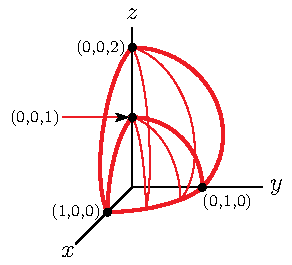
\includegraphics{fig/OE06A_8b.pdf}
\end{center}

(b) $\frac{11\pi}{6}$
\end{answer}

\begin{solution}
(a)
First observe that both boundaries of $E$, namely $\rho=1$ and 
$\rho= 1 + \cos\varphi$, are independent of the spherical coordinate
$\theta$. So $E$ is invariant under rotations about the $z$--axis.
To sketch $E$ we
\begin{itemize}
\item
first sketch the part of the boundary of $E$ with $\theta=0$
(i.e. in the half of the $xz$--plane with $x>0$), and then

\item
rotate about the $z$--axis.
\end{itemize}
The part of the boundary of $E$ with $\theta=0$ (i.e. 
in the half--plane $y=0$, $x\ge 0$), consists of two curves.
\begin{itemize}
\item
$\rho=1+\cos\varphi$, $\theta=0$:\ \ \ 
\begin{itemize}
\item When $\varphi=0$ (i.e. on the positive $z$--axis),
We have $\cos\varphi =1$ and hence $\rho=2$.  So this curve starts
at $(0,0,2)$.
\item 
As $\varphi$ increases $\cos\varphi$, and hence $\rho$,
decreases.
\item
When $\varphi$ is $\frac{\pi}{2}$ (i.e. in the $xy$--plane),
we have $\cos\varphi =0$ and hence $\rho=1$.
\item 
When $\frac{\pi}{2}<\varphi\le \pi$, we have $\cos\varphi<0$ and hence
$\rho<1$. All points in $E$ are required to obey $\rho\ge 1$. So
this part of the boundary stops at the point $(1,0,0)$ in the $xy$--plane.
\item 
The curve $\rho=1+\cos\varphi$, $\theta=0$, $0\le\varphi\le\frac{\pi}{2}$
is sketched in the figure on the left below. It is the outer curve from
$(0,0,2)$ to $(1,0,0)$.
 
\end{itemize}
 
\item
$\rho=1$, $\theta=0$:\ \ \ 

\begin{itemize}
\item
The surface $\rho=1$ is the sphere of radius $1$ centred on the origin.

\item
As we observed above, the conditions $1\le\rho\le 1+\cos\varphi$
force $0\le\varphi\le\frac{\pi}{2}$, i.e. $z\ge 0$.

\item 
The sphere $\rho=1$ intersects the quarter plane $y=0$, $x\ge 0$, $z\ge 0$, 
in the quarter circle centred on the origin that starts at $(0,0,1)$ 
on the $z$--axis and ends at $(1,0,0)$ in the $xy$--plane.

\item
The curve $\rho=1$, $\theta=0$, $0\le\varphi\le\frac{\pi}{2}$
is sketched in the figure on the left below. It is the inner curve from
$(0,0,1)$ to $(1,0,0)$.

\end{itemize}
To get $E$, rotate the shaded region in the figure on the left below
about the $z$-axis. The part of $E$ in the first octant is sketched
in the figure on the right below. The part of $E$ in the $xz$--plane 
(with $x\ge 0$) is lightly shaded and the part of $E$ in the $yz$--plane 
(with $y\ge 0$) is shaded a little more darkly.

\begin{center}
     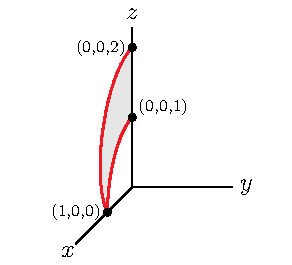
\includegraphics{fig/OE06A_8aa.pdf}\qquad
     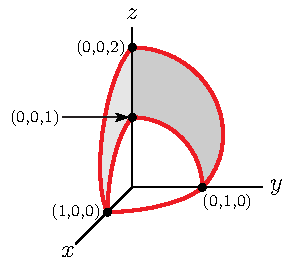
\includegraphics{fig/OE06A_8bb.pdf}
\end{center}
\end{itemize}

(b) In $E$
\begin{itemize}
\item
$\varphi$ runs from $0$ (i.e. the positive $z$--axis) to $\frac{\pi}{2}$
(i.e. the $xy$--plane).
\item
For each $\varphi$ in that range $\rho$ runs from $1$ to 
$1+\cos\varphi$ and $\theta$ runs from $0$ to $2\pi$.
\item
In spherical coordinates $\dee{V} = \rho^2\,\sin\varphi\,\dee{\rho}\,
     \dee{\theta}\,\dee{\varphi}$.
\end{itemize}
So
\begin{align*}
\text{Volume}(E)
&=\int_0^{\pi/2}\dee{\varphi} \int_1^{1+\cos\varphi}\dee{\rho}
\int_0^{2\pi}\dee{\theta}\ \rho^2\sin\varphi \\
&=2\pi \int_0^{\pi/2}\dee{\varphi}\ \sin\varphi\ 
        \frac{(1+\cos\varphi)^3-1^3}{3} \\
&=-\frac{2\pi}{3} \int_2^1 \big(u^3-1\big)\ \dee{u}
\qquad\text{with }u=1+\cos\varphi,\ \dee{u}=-\sin\varphi\,\dee{\varphi} \\
&= -\frac{2\pi}{3}\left[\frac{u^4}{4}-u\right]_2^1 \\
&=-\frac{2\pi}{3} \left[\frac{1}{4}-1-4+2\right] \\
&=\frac{11 \pi}{6}
\end{align*}
\end{solution}


%%%%%%%%%%%%%%%%%%%%%%%%%%%%%%%%
\begin{question}[M200 2006D] %6b
Use spherical coordinates to evaluate the integral
\begin{equation*}
I=\tripInt_D z\ \dee{V}
\end{equation*}
where $D$ is the solid enclosed by the cone $z = \sqrt{x^2 + y^2}$
and the sphere $x^2 + y^2 + z^2 = 4$. That is, $(x,y,z)$ is in $D$ if and only if $\sqrt{x^2 + y^2}\le z$ and $x^2 + y^2 + z^2 \le 4$.
\end{question}

%\begin{hint}
%
%\end{hint}

\begin{answer}
$2\pi$
\end{answer}

\begin{solution}
Recall that in spherical coordinates,
\begin{align*}
x&=\rho\sin\varphi\cos\theta \\
y&=\rho\sin\varphi\sin\theta \\
z&=\rho\cos\varphi \\
x^2+y^2 &=\rho^2\sin^2\varphi
\end{align*}
so that $x^2+y^2+z^2= 4$ becomes $\rho = 2$,
and $\sqrt{x^2+y^2}= z$ becomes
\begin{align*}
\rho\sin\varphi = \rho\cos\varphi 
\iff
\tan\varphi= 1
\iff
\varphi=\frac{\pi}{4}
\end{align*}
Here is a sketch of the $y=0$ cross--section of $D$.
\begin{center}
     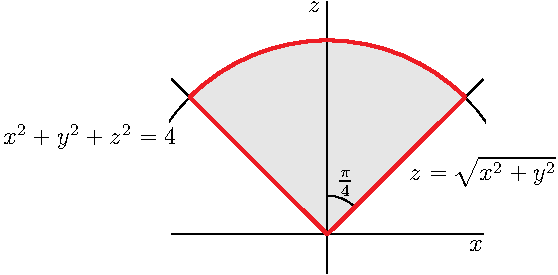
\includegraphics[scale=1.0]{fig/OE06D_6b.pdf}
\end{center}
Looking at the figure above, we see that, on $D$
\begin{itemize}
\item 
  $\varphi$ runs from $0$ (the positive $z$--axis) to
    $\frac{\pi}{4}$ (on the cone), and
\item
  for each $\varphi$ is that range, $\rho$ runs from $0$  to $2$
  and $\theta$ runs from $0$ to $2\pi$.
\end{itemize}
So
\begin{align*}
D&=\Set{(\rho\sin\varphi\cos\theta,\rho\sin\varphi\sin\theta,\rho\cos\varphi)}
 {0\le\varphi\le\nicefrac{\pi}{4},\ 
     0\le \theta\le 2\pi,\ \rho\le 2}
\end{align*}
and, as $\dee{V} =\rho^2\sin\varphi\,\dee{\rho}\,\dee{\theta}\,\dee{\varphi}$,
\begin{align*}
I&= \int_0^{\pi/4}\dee{\varphi}\int_0^{2\pi}\dee{\theta}
            \int_0^{2}\dee{\rho}\ 
             \rho^2\sin\varphi\ \overbrace{\rho\cos\varphi}^{z} \\
&= \int_0^{\pi/4}\dee{\varphi}\int_0^{2\pi}\dee{\theta}
            \int_0^{2}\dee{\rho}\ 
                  \rho^3\sin\varphi\,\cos\varphi \\
&= 2\pi\ \frac{2^4}{4} \int_0^{\pi/4}\dee{\varphi}\ \sin\varphi\,\cos\varphi \\
&= 2\pi\ \frac{2^4}{4}\left[\frac{\sin^2\varphi}{2}\right]_0^{\pi/4} \\
&= 2\pi
\end{align*}
\end{solution}

%%%%%%%%%%%%%%%%%%%%%%%%%%%%%%%%%%%%%%%%%
\begin{question}
Use spherical coordinates to find
\begin{enumerate}[(a)]
\item 
The volume inside the cone $z=\sqrt{x^2+y^2}$ and inside the sphere
$x^2+y^2+z^2=a^2$.
\item 
$\tripInt_R x\, \dee{V}$ and $\tripInt_R z\, \dee{V}$ over the
part of the sphere of radius $a$ that lies in the first octant.
\item
The mass of a spherical planet of radius $a$ whose density at
distance $\rho$ from the center is $\de=A/(B+\rho^2)$. 
\item
The volume enclosed by $\ \rho=a(1-\cos\varphi).$ Here $\rho$ and $\varphi$ 
refer to the usual spherical coordinates.
\end{enumerate}
\end{question}

%\begin{hint}
%
%\end{hint}

\begin{answer}
(a) $2\pi\frac{a^3}{3}\big(1-\frac{1}{\sqrt{2}}\big)$\qquad
(b) $\frac{\pi a^4}{16}$\qquad
(c) $4\pi A\big(a-\sqrt{B}\tan^{-1}\frac{a}{\sqrt{B}}\big)$\qquad
(d) $\frac{8}{3}\pi a^3$
\end{answer}

\begin{solution}
(a)
Recall that in spherical coordinates,
\begin{align*}
x&=\rho\sin\varphi\cos\theta \\
y&=\rho\sin\varphi\sin\theta \\
z&=\rho\cos\varphi \\
x^2+y^2 &=\rho^2\sin^2\varphi
\end{align*}
so that $x^2+y^2+z^2= a^2$ becomes $\rho = a$,
and $\sqrt{x^2+y^2}= z$ becomes
\begin{align*}
\rho\sin\varphi = \rho\cos\varphi 
\iff
\tan\varphi= 1
\iff
\varphi=\frac{\pi}{4}
\end{align*}
Here is a sketch of the $y=0$ cross--section of the specified region.
\begin{center}
     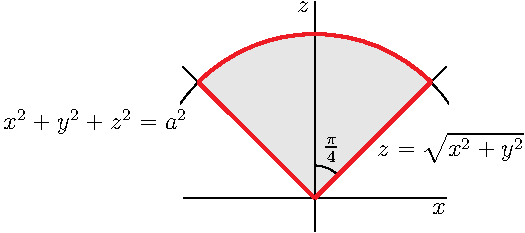
\includegraphics{fig/coneSphere.pdf}
\end{center}
Looking at the figure above, we see that, on that region,
\begin{itemize}
\item 
  $\varphi$ runs from $0$ (the positive $z$--axis) to
    $\frac{\pi}{4}$ (on the cone), and
\item
  for each $\varphi$ is that range, $\rho$ runs from $0$  to $a$
  and $\theta$ runs from $0$ to $2\pi$.
\end{itemize}
so that
\begin{align*}
\text{Volume} 
&= \int_{0}^{a}\dee{\rho}  \int_{0}^{2\pi} \dee{\theta}
\int_0^{{\pi\over 4}}\dee{\varphi}\ \rho^2\sin\varphi
= \Big\{\int_{0}^{a}\dee{\rho}\ \rho^2  \Big\}\Big\{\int_{0}^{2\pi} \dee{\theta}\Big\}\Big\{
\int_0^{{\pi\over 4}}\dee{\varphi}\ \sin\varphi\Big\} \\
&= \frac{a^3}{3}\ 2\pi\ \Big[-\cos\varphi\Big]_0^{{\pi\over 4}}
=2\pi\frac{a^3}{3}\left(1-\frac{1}{\sqrt{2}}\right)
\end{align*}

(b) The part of the sphere in question is
\begin{align*}
R&=\Set{(x,y,z)}{x^2+y^2+z^2\le a^2,\ x\ge0,\ y\ge 0,\ z\ge 0} \\
 &=\Set{(\rho\sin\varphi\cos\theta\,,\,
         \rho\sin\varphi\sin\theta\,,\,
         \rho\cos\varphi)}{\rho\le a,\ 0\le\varphi\le\tfrac{\pi}{2},
             \ 0\le\theta\le\tfrac{\pi}{2}} 
\end{align*}
By symmetry, the two specified integrals are equal, and are
\begin{align*}
 \int_{0}^{a}\dee{\rho}\ \rho^2 \int_0^{{\pi\over 2}}\dee{\varphi}\ \sin\varphi
\int_{0}^{{\pi\over 2}} \dee{\theta}\ \overbrace{\rho\cos\varphi}^{z}
&=\frac{a^4}{4}\frac{\pi}{2} \int_0^{{\pi\over 2}}\dee{\varphi}\ 
\sin\varphi\cos\varphi \\
&=\frac{\pi a^4}{8} \int_0^{1}\dee{t}\ t\qquad\hbox{ where $t=\sin\varphi$,
$\dee{t}=\cos\varphi\,\dee{\varphi}$} \\
&=\frac{\pi a^4}{16}
\end{align*}

(c) The planet in question is
\begin{align*}
P&=\Set{(x,y,z)}{x^2+y^2+z^2\le a^2} \\
 &=\Set{(\rho\sin\varphi\cos\theta\,,\,
         \rho\sin\varphi\sin\theta\,,\,
         \rho\cos\varphi)}{\rho\le a,\ 0\le\varphi\le\pi,
             \ 0\le\theta\le2\pi} 
\end{align*}
So the
\begin{align*}
\text{mass}
&= \int_{0}^{a}\dee{\rho}\ \rho^2 \int_0^{\pi}\dee{\varphi}\ \sin\varphi
\int_{0}^{2\pi} \dee{\theta}\ \overbrace{\frac{A}{B+\rho^2}}^{\rm density}
=2\pi A\Big\{ \int_0^{\pi}\dee{\varphi}\ \sin\varphi\Big\}
\Big\{\int_{0}^{a}\dee{\rho}\ \frac{\rho^2}{B+\rho^2} \Big\} \\
&=4\pi A\int_{0}^{a}\dee{\rho}\ \left(1-\frac{B}{B+\rho^2} \right) \\
&=4\pi Aa-4\pi A\sqrt{B}\int_{0}^{a/\sqrt{B}}\dee{s}\ \frac{1}{1+s^2} 
\qquad\hbox{ where $\rho=\sqrt{B}\,s$,
$\dee{\rho}=\sqrt{B}\,\dee{s}$} \\
&=4\pi A\left(a-\sqrt{B}\tan^{-1}\frac{a}{\sqrt{B}}\right)
\end{align*}

(d)  Observe that
\begin{itemize}
\item
when $\varphi=0$ (i.e. on the positive $z$--axis), $\cos\varphi=1$ so that
        $\rho=a(1-\cos\varphi)=0$ and
\item
as $\varphi$ increases from $0$ to $\frac{\pi}{2}$, $\cos\varphi$ decreases
         so that $\rho=a(1-\cos\varphi)$ increases and
\item
when $\varphi=\frac{\pi}{2}$ (i.e. on the $xy$--plane), $\cos\varphi=0$ so that
       $\rho=a(1-\cos\varphi)=a$ and
\item
as $\varphi$ increases from  $\frac{\pi}{2}$ to $\pi$, $\cos\varphi$
      continues to decrease so that
          $\rho=a(1-\cos\varphi)$ increases still more and
\item
when $\varphi=\pi$ (i.e. on the negative $z$--axis), $\cos\varphi=-1$ so that
        $\rho=a(1-\cos\varphi)=2a$
\end{itemize}
So we have the following sketch of the intersection of the specified 
volume with the right half of the $yz$--plane.
\begin{center}
     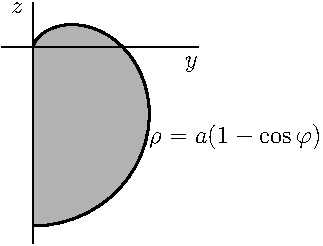
\includegraphics{fig/domain3d.pdf}
\end{center}
The volume in question is invariant under rotations about
the $z$--axis so that
\begin{align*}
\text{Volume}
&= \int_{0}^{2\pi} \dee{\theta}\int_0^{\pi}\dee{\varphi}\ \sin\varphi\int_{0}^{a(1-\cos\varphi)}\dee{\rho}\ \rho^2 
%\qquad\smash{\figplace{domain3d}{0 in}{-0.6 in}} 
\\
&=2\pi\frac{a^3}{3} \int_0^{\pi}\dee{\varphi}\ \sin\varphi(1-\cos\varphi)^3 \\
&=2\pi\frac{a^3}{3} \int_0^2\dee{t}\ t^3
\qquad\hbox{ where $t=1-\cos\varphi$, $\dee{t}=\sin\varphi\,\dee{\varphi}$} \\
&=2\pi\ \frac{a^3}{3}\ \frac{2^4}{4}
=\frac{8}{3}\pi a^3
\end{align*}
\end{solution}


%%%%%%%%%%%%%%%%%%%%%%%%%%%%%%%%
\begin{question}[M200 2008A] %4
Consider the hemispherical shell bounded by the spherical surfaces
\begin{equation*}
x^2 + y^2 + z^2 = 9\qquad\text{and}\qquad
x^2 + y^2 + z^2 = 4
\end{equation*}
and above the plane $z = 0$. Let the shell have constant density $D$. 
\begin{enumerate}[(a)]
\item
Find the mass of the shell.

\item
Find the location of the center of mass of the shell.
\end{enumerate}
\end{question}

%\begin{hint}
%
%\end{hint}

\begin{answer}
(a) $\frac{38}{3}\pi D$

(b)
$\bar x = \bar y=0$\qquad
$\bar z =\frac{195}{152} \approx 1.28$
\end{answer}

\begin{solution}
Let's use $H$ to denote the hemispherical shell.
On that shell, the spherical coordinate $\varphi$ runs from $0$
(on the $z$--axis) to $\pi/2$ (on the $xy$--plane, $z=0$)
and the spherical coordinate $\rho$ runs from $2$, on $x^2+y^2+z^2=4$,
to $3$, on $x^2+y^2+z^2=9$. So, in spherical coordinates,
\begin{align*}
H=\Set{
(\rho\sin\varphi\cos\theta\,,\,\rho\sin\varphi\sin\theta\,,\,\rho\cos\varphi)}
{2\le \rho\le 3,\ 0\le\varphi\le\pi/2,\ 0\le\theta\le 2\pi}
\end{align*}

(a) In spherical coordinates 
$\dee{V}=\rho^2\sin\varphi\ \dee{\rho}\,\dee{\varphi}\,\dee{\theta}$,
so that, as the density is the constant $D$,
\begin{align*}
\text{Mass}(H)
&=\int_2^3\dee{\rho} \int_0^{2\pi}\dee{\theta}\int_0^{\pi/2}\dee{\varphi}\ 
           D\ \rho^2\sin\varphi \\
&=D\ \left[\int_2^3\dee{\rho}\ \rho^2\right]\ 
     \left[\int_0^{2\pi}\dee{\theta}\right]\ 
     \left[\int_0^{\pi/2}\dee{\varphi}\ \sin\varphi\right] \\
&= D\left[\frac{3^3}{3}-\frac{2^3}{3}\right]\ 
     \big[2\pi\big]\ \big[\cos 0 -\cos(\pi/2)\big] \\
&=\frac{38}{3}\pi D
\end{align*}

\goodbreak
We could have gotten the same result by expressing the mass as
\begin{itemize}
\item
one half, times
\item
the density $D$, times
\item
the difference between 
the volume of a sphere of radius $3$ and a sphere of radius $2$.
\end{itemize}
That is
\begin{align*}
\text{Mass}(H) =\frac{1}{2}D\left[\frac{4}{3}\pi 3^3-\frac{4}{3}\pi 2^3\right]
               =\frac{38}{3}\pi D
\end{align*}

(b) By definition, the centre of mass is $(\bar x,\bar y,\bar z)$
where $\bar x$, $\bar y$ and $\bar z$ are the weighted averages of
$x$, $y$ and $z$, respectively, over $H$. That is
\begin{align*}
\bar x =\frac{\tripInt_H x\,D\,\dee{V}}{\tripInt_H D\,\dee{V}}\qquad
\bar y =\frac{\tripInt_H y\,D\,\dee{V}}{\tripInt_H D\,\dee{V}}\qquad
\bar z =\frac{\tripInt_H z\,D\,\dee{V}}{\tripInt_H D\,\dee{V}}
\end{align*}
As $H$ is invariant under reflection in the $yz$--plane (i.e. under
$x\rightarrow-x$) we have $\bar x=0$.
As $H$ is also invariant under reflection in the $xz$--plane (i.e. under
$y\rightarrow-y$) we have $\bar y=0$.
So we just have to find $\bar z$. We have already found the denominator in part 
(a), so we just have evaluate the numerator
\begin{align*}
\tripInt_H z\,D\,\dee{V}
&=\int_2^3\dee{\rho} \int_0^{2\pi}\dee{\theta}\int_0^{\pi/2}\dee{\varphi}\ 
           D\ \rho^2\sin\varphi\ \overbrace{\rho\cos\varphi}^{z} \\
&=D\ \left[\int_2^3\dee{\rho}\ \rho^3\right]\ 
     \left[\int_0^{2\pi}\dee{\theta}\right]\ 
     \left[\int_0^{\pi/2}\dee{\varphi}\ \sin\varphi\ \cos\varphi\right] \\
&= D\left[\frac{3^4}{4}-\frac{2^4}{4}\right]\ 
     \big[2\pi\big]\ 
     \left[\frac{1}{2}\sin^2\frac{\pi}{2} -\frac{1}{2}\sin^2 0\right] \\
&=\frac{81-16}{4}\pi D
=\frac{65}{4}\pi D
\end{align*}
All together
\begin{align*}
\bar x = \bar y=0\qquad
\bar z =\frac{\frac{65}{4}\pi D}{\frac{38}{3}\pi D}
       =\frac{195}{152}
       \approx 1.28
\end{align*}
\end{solution}

%%%%%%%%%%%%%%%%%%%%%%%%%%%%%%%%
\begin{question}[M200 2008D] %8
Let
\begin{equation*}
I = \tripInt_T xz\ \dee{V}
\end{equation*}
where $T$ is the eighth of the sphere $x^2 + y^2 + z^2 \le 1$ with 
$x,y,z \ge 0$.
\begin{enumerate}[(a)]
\item
Sketch the volume $T$.

\item
Express $I$ as a triple integral in spherical coordinates.

\item
Evaluate $I$ by any method.

\end{enumerate}
\end{question}

%\begin{hint}
%
%\end{hint}

\begin{answer}
(a)
\begin{center}
     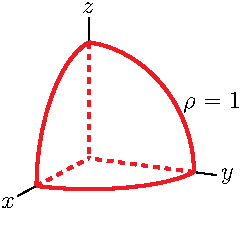
\includegraphics{fig/OE08D_8.pdf}
\end{center}

(b) $I=\int_0^{\pi/2}\dee{\varphi}\int_0^{\pi/2}\dee{\theta}\int_0^1\dee{\rho}\ 
         \rho^4\sin^2\varphi\cos\varphi\ \cos\theta$

(c) $\frac{1}{15}$
\end{answer}

\begin{solution}
(a) Here is a sketch
\begin{center}
     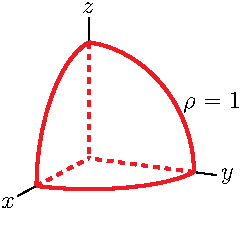
\includegraphics{fig/OE08D_8.pdf}
\end{center}


(b) On $T$,
\begin{itemize}
\item
the spherical coordinate $\varphi$ runs from $0$ (the positive $z$--xis)
to $\nicefrac{\pi}{2}$ (the $xy$--plane), and
\item 
for each fixed $\varphi$ in that range,
$\theta$ runs from $0$ to $\nicefrac{\pi}{2}$, and
\item
for each fixed $\varphi$ and $\theta$, the spherical coordinate
$\rho$ runs from $0$ to $1$.
\item
In spherical coordinates 
  $\dee{V}=\rho^2\,\sin\varphi\,\dee{\rho}\,\dee{\theta}\, \dee{\varphi}$
and
\begin{equation*}
   xz=\big(\rho\sin\varphi\cos\theta\big)\big(\rho\cos\varphi\big)
      =\rho^2 \sin\varphi\ \cos\varphi\ \cos\theta
\end{equation*}
\end{itemize}
So
\begin{align*}
I=\int_0^{\pi/2}\dee{\varphi}\int_0^{\pi/2}\dee{\theta}\int_0^1\dee{\rho}\ 
         \rho^4\sin^2\varphi\cos\varphi\ \cos\theta
\end{align*} 

(c) In spherical coordinates,
\begin{align*}
I&=  \left[\int_0^{\pi/2}\dee{\varphi}\ \sin^2\varphi\cos\varphi\right]
    \left[\int_0^{\pi/2}\dee{\theta}\ \cos\theta\right]
     \left[\int_0^1\dee{\rho}\ \rho^4\right] \\
 &=\left[\frac{\sin^3\varphi}{3}\right]_0^{\pi/2}
    \left[\sin\theta\right]_0^{\pi/2}
     \left[\frac{\rho^5}{5}\right]_0^1 \\
 &=\frac{1}{15}
\end{align*}
\end{solution}

%%%%%%%%%%%%%%%%%%%%%%%%%%%%%%%%
\begin{question}[M200 2010D] %8
Evaluate $W = \tripInt_Q xz\ \dee{V}$, where $Q$ is an eighth of the sphere 
$x^2 + y^2 + z^2 \le 9$ with $x$, $y$, $z \ge 0$.
\end{question}

%\begin{hint}
%
%\end{hint}

\begin{answer}
$\frac{81}{5}$
\end{answer}

\begin{solution}
We'll use spherical coordinates.
On $Q$, 
\begin{itemize}
\item
the spherical coordinate $\varphi$ runs from $0$
(the positive $z$--axis) to $\frac{\pi}{2}$ (the $xy$--plane), 
\item
the spherical coordinate $\theta$ runs from $0$ (the half of the 
$xz$--plane with $x\ge 0$) to $\frac{\pi}{2}$ (the half of the 
$yz$--plane with $y\ge 0$) and
\item
the spherical coordinate $\rho$ runs from $0$ to $3$.
\end{itemize}
As $\dee{V}=\rho^2\sin\varphi\,\dee{\rho}\,\dee{\theta}\,\dee{\varphi}$,
\begin{align*}
W&= \tripInt_Q xz\ \dee{V}
=\int_0^3 \dee{\rho} \int_0^{\pi/2}\dee{\theta}\int_0^{\pi/2}\dee{\varphi}
\ \rho^2\sin\varphi\ \overbrace{\rho\sin\varphi\cos\theta}^{x}
  \overbrace{\rho\cos\varphi}^{z} \\
&=\int_0^3 \dee{\rho} \int_0^{\pi/2}\dee{\theta}
\ \rho^4\cos\theta\left[\frac{\sin^3\varphi}{3}\right]
        _{\varphi=0}^{\varphi=\pi/2} \\
&=\frac{1}{3}\int_0^3 \dee{\rho}\ \rho^4\Big[\sin\theta\Big]_0^{\pi/2} \\
&=\frac{3^5}{15}=\frac{81}{5}
\end{align*}
\end{solution}

%%%%%%%%%%%%%%%%%%%%%%%%%%%%%%%%
\begin{question}[M200 2012A] %10
Evaluate $\tripInt_{\bbbr^3}  {\big[1+{(x^2+y^2+z^2)}^3\big]}^{-1}\ \dee{V}$.
\end{question}

%\begin{hint}
%
%\end{hint}

\begin{answer}
$\frac{2\pi^2}{3}$
\end{answer}

\begin{solution}
Let's use spherical coordinates. This is an improper integral.
So, to be picky, we'll take the limit as $R\rightarrow\infty$
of the integral over $0\le\rho\le R$.
\begin{align*}
\tripInt_{\bbbr^3}  {\big[1+{(x^2+y^2+z^2)}^3\big]}^{-1}\ \dee{V}
&=\lim_{R\rightarrow\infty}
        \int_0^R \dee{\rho} \int_0^{2\pi}\dee{\theta} \int_0^\pi\dee{\varphi}\ 
                      \rho^2\sin\varphi\ \frac{1}{1+\rho^6} \\
&=\lim_{R\rightarrow\infty}
        \int_0^R  \dee{\rho} \int_0^{2\pi}\dee{\theta} \ 
       \frac{\rho^2}{1+\rho^6}\Big[-\cos\varphi\Big]_0^\pi \\
&=4\pi \lim_{R\rightarrow\infty}
        \int_0^R  \dee{\rho} \ \frac{\rho^2}{1+\rho^6} \\
&=\frac{4\pi}{3} \lim_{R\rightarrow\infty}
        \int_0^{R^3}  \dee{u} \ \frac{1}{1+u^2}\qquad
\text{with }u=\rho^3,\ \dee{u}=3\rho^2\,\dee{\rho} \\
&=\frac{4\pi}{3}\lim_{R\rightarrow\infty}\Big[\arctan u\Big]_0^{R^3} \\
&=\frac{2\pi^2}{3}\qquad\text{since }
            \lim_{R\rightarrow\infty}\arctan R^3=\frac{\pi}{2}
\end{align*}
\end{solution}

%%%%%%%%%%%%%%%%%%%%%%%%%%%%%%%%
\begin{question}[M200 2012D] %10
Evaluate
\begin{equation*}
\int_{-1}^1 \int_{-\sqrt{1-x^2}}^{\sqrt{1-x^2}}  
           \int_{1-\sqrt{1-x^2-y^2}}^{1+\sqrt{1-x^2-y^2}}
   (x^2+y^2+z^2)^{5/2}  \ \dee{z}\,\dee{y}\,\dee{x}
\end{equation*}
by changing to spherical coordinates.
\end{question}

%\begin{hint}
%
%\end{hint}

\begin{answer}
$\frac{64\pi}{9}$
\end{answer}

\begin{solution}
On the domain of integration 
\begin{itemize}
\item
$x$ runs from $-1$ to $1$. 
\item
For each fixed $x$ in that range, $y$ runs from $-\sqrt{1-x^2}$ to
$\sqrt{1-x^2}$. In inequalities, that is $-\sqrt{1-x^2}\le y\le \sqrt{1-x^2}$,
which is equivalent to $x^2+y^2\le 1$.
\item
For each fixed $(x,y)$ obeying $x^2+y^2\le 1$, $z$ runs from
$1-\sqrt{1-x^2-y^2}$ to $1+\sqrt{1-x^2-y^2}$.
In inequalities, that is $1-\sqrt{1-x^2-y^2}\le z\le 1+\sqrt{1-x^2-y^2}$,
which is equivalent to $x^2+y^2+(z-1)^2\le 1$. 
\end{itemize}
So the domain of integration is
\begin{equation*}
V = \Set{(x,y,z)}{x^2+y^2+(z-1)^2\le 1}
\end{equation*}
In spherical coordinates, the  condition $x^2+y^2+(z-1)^2\le 1$ is
\begin{align*}
&(\rho\sin\varphi\cos\theta)^2
+(\rho\sin\varphi\sin\theta)^2
+(\rho\cos\varphi-1)^2\le 1 \\
&\iff
\rho^2\sin^2\varphi + (\rho\cos\varphi-1)^2\le 1 \\
&\iff 
\rho^2\sin^2\varphi + \rho^2\cos^2\varphi -2 \rho\cos\varphi +1 \le 1 \\
&\iff
\rho^2\le 2\rho\cos\varphi \\
&\iff
\rho\le 2\cos\varphi
\end{align*}
Note that $V$ is contained in the upper half, $z\ge 0$, of $\bbbr^3$
and that the $xy$--plane in tangent to $V$. So as $(x,y,z)$ runs over $V$,
the spherical coordinate $\varphi$ runs from $0$ (the positive $z$--axis) 
to $\nicefrac{\pi}{2}$ (the $xy$--plane). Here is a sketch of the side view
of $V$.

\begin{center}
     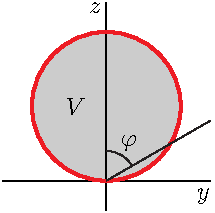
\includegraphics{fig/OE12D_10.pdf}
\end{center}

 
As $\dee{V} = \rho^2\sin\varphi\ \dee{\rho}\,\dee{\varphi}\,\dee{\theta}$
and $\big(x^2+y^2+z^2\big)^{5/2}=\rho^5$, the integral is
\begin{align*}
\int_{-1}^1 \int_{-\sqrt{1-x^2}}^{\sqrt{1-x^2}}  
           \int_{1-\sqrt{1-x^2-y^2}}^{1+\sqrt{1-x^2-y^2}}
   (x^2+y^2+z^2)^{5/2}  \ \dee{z}\,\dee{y}\,\dee{x}
&=\int_0^{2\pi}\dee{\theta}\int_0^{\pi/2}\dee{\varphi}
       \int_0^{2\cos\varphi}\dee{\rho}\ \rho^2\sin\varphi
        \ \rho^5 \\
&=\int_0^{2\pi}\dee{\theta}\int_0^{\pi/2}\dee{\varphi}
       \ \frac{2^8\cos^8\varphi}{8}\sin\varphi \\
&=32\int_0^{2\pi}\dee{\theta}\ \left[-\frac{\cos^9\varphi}{9}\right]_0^{\pi/2}
  \\
&=\frac{32}{9}(2\pi)
=\frac{64\pi}{9}
\end{align*}
\end{solution}

%%%%%%%%%%%%%%%%%%%%%%%%%%%%%%%%%%%%%%%%%
\begin{question}
Evaluate the volume of a circular cylinder of radius $a$ and height $h$ by means of an integral in spherical coordinates.
\end{question}

%\begin{hint}
%
%\end{hint}

\begin{answer}
$\pi a^2h$
\end{answer}

\begin{solution}
The top of the cylinder has equation $z=h$, i.e. $\rho\cos\varphi=h$.
The side of the cylinder has equation $x^2+y^2=a^2$, i.e. $\rho\sin\varphi=a$.
The bottom of the cylinder has equation $z=0$, i.e. $\varphi=\frac{\pi}{2}$.
\begin{center}
     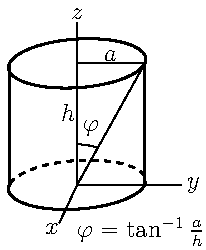
\includegraphics{fig/cylinder1.pdf}\qquad
     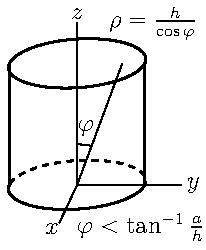
\includegraphics{fig/cylinder2.pdf}\qquad
     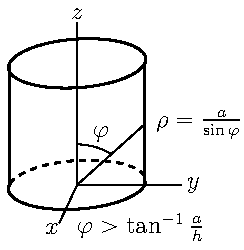
\includegraphics{fig/cylinder3.pdf}
\end{center}
For each fixed $\varphi$, $\theta$ runs from $0$ to $2\pi$ and $\rho$ 
runs from $0$
to either $\frac{h}{\cos\varphi}$ (at the top of the can,
if $\varphi<\tan^{-1}\frac{a}{h}$)
or $\frac{a}{\sin\varphi}$ (at the side of the can, if $\varphi>\tan^{-1}\frac{a}{h}$). So the
\begin{align*}
\text{Volume} 
&= \int_{0}^{\tan^{-1}{a\over h}} \dee{\varphi} \int_{0}^{2\pi} \dee{\theta}
\int_0^{h/\cos\varphi}\dee{\rho}\ \rho^2\sin\varphi
+\int_{\tan^{-1}{a\over h}}^{{\pi\over 2}} \dee{\varphi} \int_{0}^{2\pi} \dee{\theta}
\int_0^{a/\sin\varphi}\dee{\rho}\ \rho^2\sin\varphi \\
&= 2\pi\int_{0}^{\tan^{-1}{a\over h}} \dee{\varphi} 
\ \frac{h^3\sin\varphi}{3\cos^3\varphi}
+2\pi\int_{\tan^{-1}{a\over h}}^{{\pi\over 2}} \dee{\varphi} 
\ \frac{a^3\sin\varphi}{3\sin^3\varphi} \\
&=2\pi\Big\{\int_0^{{a\over h}}\dee{t}\ \frac{h^3}{3}t
-\int^0_{{h\over a}}\dee{s}\ \frac{a^3}{3}\Big\} \\
&\hskip1in\hbox{ where $t=\tan\varphi$, $\dee{t}=\sec^2\varphi\,\dee{\varphi}$,
$s=\cot\varphi$, $\dee{s}=-\csc^2\varphi\,\dee{\varphi}$} \\
&=2\pi\left\{\frac{h^3}{3}\,\frac{1}{2}\left(\frac{a}{h}\right)^2
+\frac{a^3}{3}\,\frac{h}{a}\right\}
=2\pi\left\{\frac{ah^2}{6}+\frac{a^2h}{3}\right\}
=\pi a^2h
\end{align*}
\end{solution}

%%%%%%%%%%%%%%%%%%%%%%%%%%%%%%%%%%%%%%%%%
\begin{question} [M200 2003A] % 7a
Let $B$ denote the region inside the sphere $x^2+y^2+z^2=4$
and above the cone $x^2+y^2=z^2$. Compute the moment of inertia
\begin{equation*}
\tripInt_B z^2\,\dee{V}
\end{equation*}
\end{question}

%\begin{hint}
%
%\end{hint}

\begin{answer}
$\frac{64}{15}\pi\big(1-\frac{1}{2\sqrt{2}}\big)\approx 8.665 $
\end{answer}

\begin{solution}
In spherical coordinates,
\begin{equation*}
x=\rho\sin\varphi\cos\theta\qquad y=\rho\sin\varphi\sin\theta\qquad z=\rho\cos\varphi
\end{equation*}
so that the sphere $x^2+y^2+z^2=4$ is $\rho^2=4$ or $\rho=2$ and the 
cone $x^2+y^2=z^2$ is $\rho^2\sin^2\varphi=\rho^2\cos^2\varphi$ or $\tan\varphi=\pm1$
or $\varphi=\frac{\pi}{4},\ \frac{3\pi}{4}$. So
\begin{align*}
\text{moment}
&=\int_0^2\dee{\rho}\int_0^{\pi/4}\dee{\varphi}\int_0^{2\pi}\dee{\theta}\ \rho^2\sin\varphi
                                           \  (\rho\cos\varphi)^2
=2\pi\int_0^2 \dee{\rho}\ \rho^4\int_0^{\pi/4}\dee{\varphi}\ \sin\varphi\cos^2\varphi\\
&=2\pi\left[\frac{\rho^5}{5}\right]_0^2
    \left[-\frac{1}{3}\cos^3\varphi\right]_0^{\pi/4}
=\frac{64}{15}\pi\left(1-\frac{1}{2\sqrt{2}}\right)\approx 8.665 
\end{align*}
\end{solution}

%%%%%%%%%%%%%%%%%%%%%%%%%%%%%%%%
\begin{question}[M200 2002A] %8
\begin{enumerate}[(a)]
\item
Evaluate $\dst\tripInt_\Om z\,\dee{V}$ where $\Om$
is the three dimensional region in the first octant $x\ge 0$, $y\ge 0$,
$z\ge 0$, occupying the inside of the sphere $x^2+y^2+z^2=1$.

\item
Use the result in part (a) to quickly determine the centroid
of a hemispherical ball given by $z\ge 0$, $x^2+y^2+z^2\le 1$.
\end{enumerate}
\end{question}

%\begin{hint}
%\end{hint}

\begin{answer}
(a) $\frac{\pi}{16}$\qquad
(b)  The centroid is $(\bar x,\bar y,\bar z)$ with 
$\bar x=\bar y=0$ and $\bar z=\frac{3}{8}$.
\end{answer}

\begin{solution}
(a) 
In spherical coordinates,
\begin{align*}
x=\rho\sin\phi\cos\theta\qquad y=\rho\sin\phi\sin\theta\qquad z=\rho\cos\phi
\end{align*}
so that
\begin{itemize}
\item
the sphere $x^2+y^2+z^2=1$ is $\rho=1$, 
\item
the $xy$-plane, $z=0$, is $\phi=\frac{\pi}{2}$, 
\item
the positive half of the $xz$-plane, $y=0$, $x>0$, is $\theta=0$ and 
\item
the positive half of the $yz$-plane, $x=0$, $y>0$, is $\theta=\frac{\pi}{2}$. 
\end{itemize}
So
\begin{align*}
\tripInt_\Om z\,\dee{V}&=
\int_0^1 \dee{\rho}\int_0^{\pi/2}d\phi\int _0^{\pi/2}\dee{\theta}\  \rho^2\sin\phi\overbrace{(\rho\cos\phi)}^{z} \\
&=\frac{\pi}{2}\int_0^1 \dee{\rho}\int_0^{\pi/2}d\phi\  \rho^3\sin\phi \cos\phi
\\
&=\frac{\pi}{2}\int_0^1 \dee{\rho}\  \rho^3\ \frac{1}{2}\sin^2\phi \Big|_0^{\pi/2}
=\frac{\pi}{4}\int_0^1 \dee{\rho}\  \rho^3
=\frac{\pi}{16}
\end{align*}

(b) The hemispherical ball given by $z\ge 0$, $x^2+y^2+z^2\le 1$
(call it $H$) has centroid $(\bar x,\bar y,\bar z)$ with 
$\bar x=\bar y=0$ (by symmetry) and
\begin{align*}
\bar z=\frac{\tripInt_H z\,\dee{V}}{\tripInt_H\,\dee{V}}
=\frac{4\tripInt_\Om z\,\dee{V}}{\half\times\frac{4}{3}\pi}
=\frac{\frac{\pi}{4}}{\frac{2\pi}{3}}
=\frac{3}{8}
\end{align*}
\end{solution}

%%%%%%%%%%%%%%%%%%%%%%%%%%%%%%%%
\begin{question}[M200 2000D] %7
Consider the top half of a ball of radius 2 centred at the
origin. Suppose that the ball has variable density equal to $9z$ units
of mass per unit volume.
\begin{enumerate}[(a)]
\item 
Set up a triple integral giving the mass of this half--ball.

\item
Find out what fraction of that mass lies inside the cone
\begin{equation*}
z=\sqrt{x^2+y^2}
\end{equation*}
\end{enumerate}
\end{question}

%\begin{hint}
%
%\end{hint}

\begin{answer}
(a) $\dst 9\int_0^2d\rho\int_0^{\pi/2}d\phi\int_0^{2\pi}d\theta\ 
            \rho^3\,\sin\phi\,\cos\phi$\qquad
(b) $\frac{1}{2}$
\end{answer}

\begin{solution}
(a) In spherical coordinates,
\begin{equation*}
x=\rho\sin\phi\cos\theta\qquad y=\rho\sin\phi\sin\theta\qquad z=\rho\cos\phi
\end{equation*}
the sphere $x^2+y^2+z^2=4$ is $\rho^2=4$ or $\rho=2$ and the 
$xy$-plane is $\phi=\frac{\pi}{2}$. So
\begin{equation*}
\text{mass}
=\int_0^2d\rho\int_0^{\pi/2}d\phi\int_0^{2\pi}d\theta\ \rho^2\sin\phi
\ \overbrace{(9 \rho\cos\phi)}^{\rm density}
\end{equation*}

(b) The mass of the half ball is
\begin{equation*}
9 \int_0^2d\rho\int_0^{\pi/2}d\phi\int_0^{2\pi}d\theta\ \rho^3\sin\phi \cos\phi
=9 \bigg[\int_0^2d\rho\ \rho^3\bigg]
  \bigg[\int_0^{\pi/2}d\phi\ \sin\phi \cos\phi\bigg]
  \bigg[\int_0^{2\pi}d\theta\bigg]
\end{equation*}
In spherical coordinates, the 
cone $x^2+y^2=z^2$ is $\rho^2\sin^2\phi=\rho^2\cos^2\phi$ or 
$\tan\phi=\pm1$ or $\phi=\frac{\pi}{4},\ \frac{3\pi}{4}$. So the mass
of the part that is inside the cone is
\begin{equation*}
9 \int_0^2d\rho\int_0^{\pi/4}d\phi\int_0^{2\pi}d\theta\ \rho^3\sin\phi \cos\phi
=9 \bigg[\int_0^2d\rho\ \rho^3\bigg]
  \bigg[\int_0^{\pi/4}d\phi\ \sin\phi \cos\phi\bigg]
  \bigg[\int_0^{2\pi}d\theta\bigg]
\end{equation*}
The fraction inside the cone is
\begin{equation*}
\frac{\int_0^{\pi/4}d\phi\ \sin\phi \cos\phi}{\int_0^{\pi/2}d\phi\ \sin\phi \cos\phi}
=\frac{\half\sin^2\phi\big|_0^{\pi/4}}{\half\sin^2\phi\big|_0^{\pi/2}}
=\frac{1}{2}
\end{equation*}
\end{solution}



%%%%%%%%%%%%%%%%%%
\subsection*{\Application}
%%%%%%%%%%%%%%%%%%

%%%%%%%%%%%%%%%%%%%%%%%%%%%%%%%%
\begin{question}[M253 2010D] %1
Find the limit or show that it does not exist
\begin{equation*}
\lim_{(x,y,z)\to(0,0,0)}\frac{xy+yz^2+xz^2}{x^2+y^2+z^4}
\end{equation*}

\end{question}

\begin{hint}
Switch to spherical coordinates.
\end{hint}

\begin{answer}
It does not exist.
\end{answer}

\begin{solution}
In spherical coordinates, $x=\rho\sin\varphi\cos\theta$, 
$y=\rho\sin\varphi\sin\theta$, $z=\rho\cos\varphi$ so that 
\begin{align*}
&\frac{\rho^2\sin^2\varphi\cos\theta\sin\theta
      +\rho^3\sin\varphi\sin\theta\,\cos^2\varphi
      +\rho^3\sin\varphi\,\cos^2\varphi}
     {\rho^2\sin^2\varphi+\rho^4\cos^4\varphi} \\
&\hskip1in 
=\frac{\sin^2\varphi\cos\theta\sin\theta
      +\rho\sin\varphi\sin\theta\,\cos^2\varphi
      +\rho\sin\varphi\cos\theta\,\cos^2\varphi}
     {\sin^2\varphi+\rho^2\cos^4\varphi}
\end{align*}
As $(x,y,z)\to (0,0,0)$, the radius $\rho\to 0$ and the second and third terms 
in the numerator and the second term in the denominator converge to $0$.
But that leaves
\begin{equation*}
\frac{\sin^2\varphi\cos\theta\sin\theta}{\sin^2\varphi}
=\cos\theta\sin\theta
\end{equation*}
which takes many different values. In particular, if we send 
$(x,y,z)\to (0,0,0)$ along either the $x$-- or $y$--axis,
that is with $z=0$ and either $x=0$ or $y=0$, then
\begin{equation*}
\frac{xy+yz^2+xz^2}{x^2+y^2+z^4}\bigg|_{\Atop{x=0\text{ or }y=0}{z=0}}=0
\end{equation*}
converges to $0$. But, if we send 
$(x,y,z)\to (0,0,0)$ along the line $y=x$, $z=0$
\begin{equation*}
\frac{xy+yz^2+xz^2}{x^2+y^2+z^4}\bigg|_{\Atop{y=x}{z=0}}=\frac{x^2}{2x^2}
=\frac{1}{2}
\end{equation*}
converges to $1/2$. So $\frac{xy+yz^2+xz^2}{x^2+y^2+z^4}$ does not 
approach a single value as  $(x,y,z)\to(0,0,0)$ and the limit does not exist.
\end{solution}

%%%%%%%%%%%%%%%%%%%%%%%%%%%%%%%%
\begin{question}[M200 2007A] %8
A certain solid $V$ is a right--circular cylinder. Its base is
the disk of radius $2$ centred at the origin in the $xy$--plane. 
It has height $2$ and density $\sqrt{x^2 + y^2}$.

A smaller solid $U$ is obtained by removing the inverted cone, 
whose base is the top surface of $V$ and whose vertex is the point $(0, 0, 0)$.

\begin{enumerate}[(a)]
\item 
    Use cylindrical coordinates to set up an integral giving the mass of $U$.
\item 
   Use spherical coordinates to set up an integral giving the mass of $U$.
\item
  Find that mass.
\end{enumerate}
\end{question}

%\begin{hint}
%
%\end{hint}

\begin{answer}
(a) $\text{Mass} = \int_0^2\dee{z}\int_0^{2\pi}\dee{\theta}\int_z^2\dee{r}\ 
                                  r^2$

(b) $\text{Mass} =  \int_{\pi/4}^{\pi/2}\dee{\varphi}\int_0^{2\pi}\dee{\theta}
            \int_0^{2/\sin\varphi}\dee{\rho}\ 
                  \rho^3\sin^2\varphi$

(c) $8\pi$
\end{answer}

\begin{solution}
The disk of radius $2$  centred at the origin in the $xy$--plane
is $x^2+y^2\le 4$. So
\begin{align*}
V&=\Set{(x,y,z)}{x^2+y^2\le 4,\ 0\le z\le 2} 
\end{align*}
The cone with vertex at the origin that contains the top edge,
$x+y^2=4$, $z=2$, of $U$ is $x^2+y^2=z^2$. So
\begin{align*}
U&=\Set{(x,y,z)}{x^2+y^2\le 4,\ 0\le z\le 2,\ x^2+y^2\ge z^2}
\end{align*} 
Here are sketches of the $y=0$ cross--section of $V$, on the left,
and $U$, on the right.
\begin{center}
     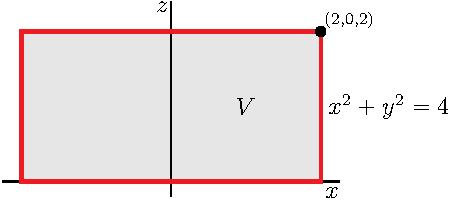
\includegraphics[scale=0.9]{fig/OE07A_8.pdf}\quad
     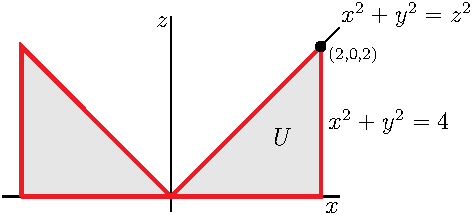
\includegraphics[scale=0.9]{fig/OE07A_8a.pdf}
\end{center}

(a) In cylindrical coordinates, $x^2+y^2\le 4$ becomes $r\le 2$
and $x^2+y^2\ge z^2$ is $r\ge |z|$, and the density is $\sqrt{x^2+y^2}=r$. 
So 
\begin{align*}
U&=\Set{(r\cos\theta,r\sin\theta,z)}{r\le 2,\ 0\le z\le 2,\ r\ge z}
\end{align*}
Looking at the figure on the left below, we see that, on $U$
\begin{itemize}
\item 
  $z$ runs from $0$ to $2$, and
\item
  for each $z$ is that range, $r$ runs from $z$ to $2$
  and $\theta$ runs from $0$ to $2\pi$.
\item $\dee{V} =r\,\dee{r}\,\dee{\theta}\,\dee{z}$
\end{itemize}
So
\begin{align*}
\text{Mass}&= \int_0^2\dee{z}\int_0^{2\pi}\dee{\theta}\int_z^2\dee{r}\ 
                  r\ \overbrace{r}^{\text{density}}
= \int_0^2\dee{z}\int_0^{2\pi}\dee{\theta}\int_z^2\dee{r}\ 
                  r^2
\end{align*}

\begin{center}
     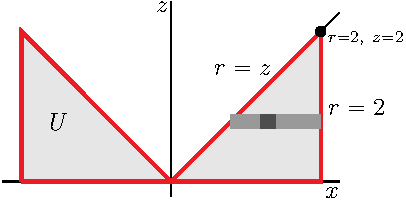
\includegraphics[scale=0.9]{fig/OE07A_8c.pdf}\quad
     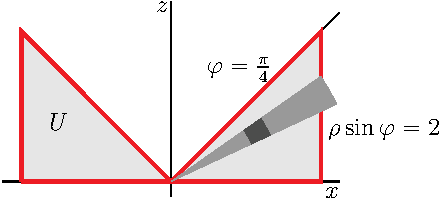
\includegraphics[scale=0.9]{fig/OE07A_8s.pdf}
\end{center}

(b)
Recall that in spherical coordinates,
\begin{align*}
x&=\rho\sin\varphi\cos\theta \\
y&=\rho\sin\varphi\sin\theta \\
z&=\rho\cos\varphi \\
x^2+y^2 &=\rho^2\sin^2\varphi
\end{align*}
so that $x^2+y^2\le 4$ becomes $\rho\sin\varphi\le 2$,
and $x^2+y^2\ge z^2$ becomes
\begin{align*}
\rho\sin\varphi \ge \rho\cos\varphi 
\iff
\tan\varphi\ge 1
\iff
\varphi\ge\frac{\pi}{4}
\end{align*}
and the density $\sqrt{x^2+y^2}=\rho\sin\varphi$. 
So 
\begin{align*}
U&=\Set{(\rho\sin\varphi\cos\theta,\rho\sin\varphi\sin\theta,\rho\cos\varphi)}
 {\nicefrac{\pi}{4}\le\varphi\le\nicefrac{\pi}{2},\ 
     0\le \theta\le 2\pi,\ \rho\sin\varphi\le 2}
\end{align*}
Looking at the figure on the right above, we see that, on $U$
\begin{itemize}
\item 
  $\varphi$ runs from $\frac{\pi}{4}$ (on the cone) to 
     $\frac{\pi}{2}$ (on the $xy$--plane), and
\item
  for each $\varphi$ is that range, $\rho$ runs from $0$ 
         to $\frac{2}{\sin\varphi}$
  and $\theta$ runs from $0$ to $2\pi$.
\item $\dee{V} =\rho^2\sin\varphi\,\dee{\rho}\,\dee{\theta}\,\dee{\varphi}$
\end{itemize}
So
\begin{align*}
\text{Mass}&= \int_{\pi/4}^{\pi/2}\dee{\varphi}\int_0^{2\pi}\dee{\theta}
            \int_0^{2/\sin\varphi}\dee{\rho}\ 
             \rho^2\sin\varphi\ \overbrace{\rho\sin\varphi}^{\text{density}} \\
&= \int_{\pi/4}^{\pi/2}\dee{\varphi}\int_0^{2\pi}\dee{\theta}
            \int_0^{2/\sin\varphi}\dee{\rho}\ 
                  \rho^3\sin^2\varphi
\end{align*}

(c) We'll use the cylindrical form.
\begin{align*}
\text{Mass}
&= \int_0^2\dee{z}\int_0^{2\pi}\dee{\theta}\int_z^2\dee{r}\ 
                  r^2 \\
&=2\pi \int_0^2\dee{z}\ \frac{8-z^3}{3} \\
&=\frac{2\pi}{3}\ \left[16-\frac{2^4}{4}\right] \\
&=8\pi
\end{align*}
\end{solution}


%%%%%%%%%%%%%%%%%%%%%%%%%%%%%%%%
\begin{question}[M200 2009A] %7
A solid is bounded below by the cone $z\!=\!\sqrt{x^2\!+\!y^2}\ $ and above  
by the sphere $x^2+y^2+z^2 = 2$. 
It has density $\de(x,y,z) = x^2 + y^2$.


\begin{enumerate}[(a)]
\item
Express the mass $M$ of the solid as a triple integral, with limits, in cylindrical coordinates.

\item
Same as (a) but in spherical coordinates.

\item
Evaluate $M$.

\end{enumerate} 
\end{question}

%\begin{hint}
%
%\end{hint}

\begin{answer}
(a) $\int_0^1\dee{r}\int_0^{2\pi}\dee{\theta}
           \int_r^{\sqrt{2-r^2}}\dee{z}\ r^3$

(b)  $\int_0^{\sqrt{2}}\dee{\rho}\int_0^{2\pi}\dee{\theta}
           \int_0^{\pi/4}\dee{\varphi}\ \rho^4\sin^3\varphi$

(c) $\pi \left[\frac{16\sqrt{2}}{15} - \frac{4}{3}\right]
     \approx 0.5503$
\end{answer}

\begin{solution}
(a)
Call the solid $V$.
In cylindrical coordinates
\begin{itemize}
\item
$x^2+y^2+z^2\le 2$ is $r^2+z^2\le 2$ and
\item
$\sqrt{x^2+y^2}\le z$ is $r\le z$ and
\item
the density $\de=r^2$, and
\item
$\dee{V}$ is $r\,\dee{r}\,\dee{\theta}\,\dee{z}$
\end{itemize}
Observe that $r^2+z^2= 2$ and $r= z$ intersect when $2r^2=2$ so that $r=z=1$.
Here is a sketch of the $y=0$ cross--section of $E$.
\begin{center}
     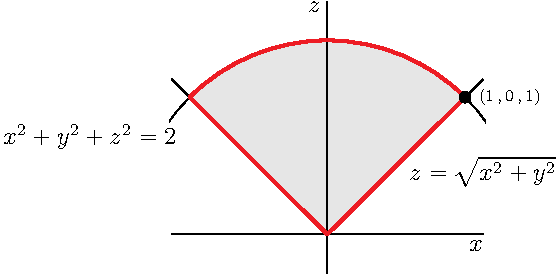
\includegraphics[scale=1.0]{fig/OE09A_7.pdf}
\end{center}
So
\begin{equation*}
V =\Set{(r\cos\theta\,,\,r\sin\theta\,,\,z)}{0\le r\le 1,\ 
                                             0\le\theta\le2\pi,\ 
                                              r\le z\le \sqrt{2-r^2}}
\end{equation*}
and
\begin{align*}
M &=\tripInt_V \rho(x,y,z)\ \dee{V} 
   =\int_0^1\dee{r}\int_0^{2\pi}\dee{\theta}
           \int_r^{\sqrt{2-r^2}}\dee{z}\ r\overbrace{(r^2)}^{\de}
   =\int_0^1\dee{r}\int_0^{2\pi}\dee{\theta}
           \int_r^{\sqrt{2-r^2}}\dee{z}\ r^3
\end{align*}

(b)
%Beware that the formulation of this question has introduced a notation
%conflict --- $\rho$ is used both for the density and for the radial 
%spherical coordinate.  We'll now start using $\rho$ \emph{just}
%for the radial spherical coordinate. 
In spherical coordinates
\begin{itemize}
\item
$x^2+y^2+z^2\le 2$ is $\rho\le\sqrt{2}$, and
\item
$\sqrt{x^2+y^2}\le z$ is $\rho\sin\varphi\le \rho\cos\varphi$,
or $\tan\varphi\le 1$ or $\varphi\le\frac{\pi}{4}$, and
\item
the density $x^2+y^2=\rho^2\sin^2\varphi$, and
\item
$\dee{V}$ is $\rho^2\sin\varphi\,\dee{\rho}\,\dee{\theta}\,\dee{\varphi}$
\end{itemize}
So
\begin{equation*}
V =\Set{(\rho\sin\varphi\cos\theta\,,\,\rho\sin\varphi\sin\theta\,,\,
          \rho\cos\varphi)}{0\le\rho\le \sqrt{2},\  0\le\theta\le2\pi,\ 
                            0\le \varphi\le \nicefrac{\pi}{4}}
\end{equation*}
and, since the integrand $x^2+y^2=\rho^2\sin^2\varphi$,
\begin{align*}
M &=\tripInt_V \big(x^2+y^2\big)\ \dee{V} 
   =\int_0^{\sqrt{2}}\dee{\rho}\int_0^{2\pi}\dee{\theta}
           \int_0^{\pi/4}\dee{\varphi}\ \rho^2\sin\varphi\ 
           \rho^2\sin^2\varphi \\
   &=\int_0^{\sqrt{2}}\dee{\rho}\int_0^{2\pi}\dee{\theta}
           \int_0^{\pi/4}\dee{\varphi}\ \rho^4\sin^3\varphi
\end{align*}


(c) We'll use the spherical coordinate form.
\begin{align*}
M &=\int_0^{\sqrt{2}}\dee{\rho}\int_0^{2\pi}\dee{\theta}
           \int_0^{\pi/4}\dee{\varphi}\ \rho^4\sin^3\varphi \\
   &=\int_0^{\sqrt{2}}\dee{\rho}\int_0^{2\pi}\dee{\theta}
           \int_0^{\pi/4}\dee{\varphi}\ \rho^4\sin\varphi
              \big[1-\cos^2\varphi\big] \\
   &=2\pi \int_0^{\sqrt{2}}\dee{\rho}\ \rho^4
                \left[-\cos\varphi +\frac{\cos^3\varphi}{3}\right]_0^{\pi/4}
    =2\pi \left[\frac{2}{3} - \frac{5}{6\sqrt{2}}\right]
                      \int_0^{\sqrt{2}}\dee{\rho}\ \rho^4 \\
    &=2\pi \frac{4\sqrt{2}}{5}\left[\frac{2}{3} - \frac{5}{6\sqrt{2}}\right]
     =\pi \left[\frac{16\sqrt{2}}{15} - \frac{4}{3}\right]
     \approx 0.5503
% 0.17516 \pi
\end{align*}

\end{solution}

%%%%%%%%%%%%%%%%%%%%%%%%%%%%%%%%
\begin{question}[M200 2009D] %8
Let
\begin{align*}
I = \tripInt_E xz\ \dee{V}
\end{align*}
where $E$ is the eighth of the sphere $x^2+y^2+z^2\le 1$ with
$x,y,z\ge 0$.
\begin{enumerate}[(a)]
\item
Express $I$ as a triple integral in spherical coordinates.

\item
Express $I$ as a triple integral in cylindrical coordinates.

\item
Evaluate $I$ by any method.
\end{enumerate}
\end{question}

%\begin{hint}
%
%\end{hint}

\begin{answer}
(a) $\int_0^{\pi/2}\dee{\varphi}\int_0^{\pi/2}\dee{\theta}\int_0^1\dee{\rho}\ 
         \rho^4\sin^2\varphi\cos\varphi\ \cos\theta$\qquad
(b) $\int_0^1\dee{z}\int_0^{\pi/2}\dee{\theta}\int_0^{\sqrt{1-z^2}}\dee{r} \ 
         r^2\,z\,\cos\theta$

(c) $\frac{1}{15}$
\end{answer}

\begin{solution}
(a)
On $E$,
\begin{itemize}
\item
the spherical coordinate $\varphi$ runs from $0$ (the positive $z$--xis)
to $\nicefrac{\pi}{2}$ (the $xy$--plane), and
\item 
for each fixed $\varphi$ in that range,
$\theta$ runs from $0$ to $\nicefrac{\pi}{2}$, and
\item
for each fixed $\varphi$ and $\theta$, the spherical coordinate
$\rho$ runs from $0$ to $1$.
\item
In spherical coordinates 
  $\dee{V}=\rho^2\,\sin\varphi\,\dee{\rho}\,\dee{\theta}\, \dee{\varphi}$
and
\begin{equation*}
   xz=\big(\rho\sin\varphi\cos\theta\big)\big(\rho\cos\varphi\big)
      =\rho^2 \sin\varphi\ \cos\varphi\ \cos\theta
\end{equation*}
\end{itemize}
So
\begin{align*}
I=\int_0^{\pi/2}\dee{\varphi}\int_0^{\pi/2}\dee{\theta}\int_0^1\dee{\rho}\ 
         \rho^4\sin^2\varphi\cos\varphi\ \cos\theta
\end{align*} 
(b)
In cylindrical coordinates, the condition $x^2+y^2+z^2\le 1$
becomes $r^2+z^2\le 1$. So, on $E$
\begin{itemize}
\item
the cylindrical coordinate $z$ runs from $0$ (in the $xy$--plane)
to $1$ (at $(0,0,1)$) and
\item
for each fixed $z$ in that range, $\theta$ runs from $0$ to $\pi/2$ and
\item
for each such fixed $z$ and $\theta$, the cylindrical coordinate
$r$ runs from $0$ to $\sqrt{1-z^2}$ (recall that $r^2+z^2\le 1$).
\item
In cylindrical coordinates 
  $\dee{V}=r\,\dee{r}\,\dee{\theta}\, \dee{z}$
and
\begin{equation*}
   xz=\big(r\cos\theta\big)\big(z\big)
      =r\,z\, \cos\theta
\end{equation*}
So
\begin{align*}
I=\int_0^1\dee{z}\int_0^{\pi/2}\dee{\theta}\int_0^{\sqrt{1-z^2}}\dee{r} \ 
         r^2\,z\,\cos\theta
\end{align*}  

 (c)
Both spherical and cylindrical integrals are straight forward to evaluate.
Here are both. First, in spherical coordinates,
\begin{align*}
I&=  \left[\int_0^{\pi/2}\dee{\varphi}\ \sin^2\varphi\cos\varphi\right]
    \left[\int_0^{\pi/2}\dee{\theta}\ \cos\theta\right]
     \left[\int_0^1\dee{\rho}\ \rho^4\right] \\
 &=\left[\frac{\sin^3\varphi}{3}\right]_0^{\pi/2}
    \left[\sin\theta\right]_0^{\pi/2}
     \left[\frac{\rho^5}{5}\right]_0^1 \\
 &=\frac{1}{15}
\end{align*}
Now in cylindrical coordinates
\begin{align*}
I&=\int_0^1\dee{z}\int_0^{\pi/2}\dee{\theta}\int_0^{\sqrt{1-z^2}}\dee{r} \ 
         r^2\,z\,\cos\theta \\
&=\frac{1}{3}\int_0^1\dee{z}\int_0^{\pi/2}\dee{\theta}\ z{(1-z^2\big)}^{3/2}\,
            \cos\theta \\
&=\frac{1}{3}\int_0^1\dee{z}\ z{(1-z^2\big)}^{3/2} \\
&=\frac{1}{3}\left[-\frac{1}{2}\ \frac{(1-z^2)^{5/2}}{5/2}\right]_0^1\\
&=\frac{1}{15}
\end{align*}

\end{itemize}
\end{solution}


%%%%%%%%%%%%%%%%%%%%%%%%%%%%%%%%
\begin{question}[M200 2010A] %8
Let
\begin{equation*}
I = \tripInt_T  (x^2+y^2)\ \dee{V}
\end{equation*}
where $T$ is the solid region bounded below by the cone 
$z =\sqrt{3x^2+3y^2}$ and above by the sphere
$x^2 + y^2 + z^2 = 9$.
\begin{enumerate}[(a)]
\item
Express $I$ as a triple integral in spherical coordinates.
\item
Express $I$ as a triple integral in cylindrical coordinates.
\item
Evaluate $I$ by any method.
\end{enumerate}
\end{question}

%\begin{hint}
%
%\end{hint}

\begin{answer}
(a) $\int_0^{3}\dee{\rho}\int_0^{2\pi}\dee{\theta}
           \int_0^{\pi/6}\dee{\varphi}\ \rho^4\sin^3\varphi$

(b) $\int_0^{3/2}\dee{r}\int_0^{2\pi}\dee{\theta}
                          \int_{\sqrt{3}\,r}^{\sqrt{9-r^2}}\dee{z}\ \ r^3$

(c) $81\pi \left[\frac{4}{5} - \frac{9\sqrt{3}}{20}\right]
     \approx 5.24$
\end{answer}

\begin{solution}
(a)
Recall that in spherical coordinates
\begin{align*}
x=\rho\,\sin\varphi\,\cos\theta\qquad
y=\rho\,\sin\varphi\,\sin\theta\qquad
z=\rho\,\cos\varphi
\end{align*}
so that 
\begin{itemize}
\item
$x^2+y^2+z^2\le 9$ is $\rho\le 3$, and
\item
$\sqrt{3x^2+3y^2}\le z$ is $\sqrt{3}\rho\sin\varphi\le \rho\cos\varphi$,
or $\tan\varphi\le \frac{1}{\sqrt{3}}$ or $\varphi\le\frac{\pi}{6}$, and
\item
the integrand $x^2+y^2=\rho^2\sin^2\varphi$, and
\item
$\dee{V}$ is $\rho^2\sin\varphi\,\dee{\rho}\,\dee{\theta}\,\dee{\varphi}$
\end{itemize}
So
\begin{equation*}
T =\Set{(\rho\sin\varphi\cos\theta\,,\,\rho\sin\varphi\sin\theta\,,\,
          \rho\cos\varphi)}{0\le\rho\le 3,\  0\le\theta\le2\pi,\ 
                            0\le \varphi\le \nicefrac{\pi}{6}}
\end{equation*}
and, 
\begin{align*}
I &=\tripInt_T \big(x^2+y^2\big)\ \dee{V} 
   =\int_0^{3}\dee{\rho}\int_0^{2\pi}\dee{\theta}
           \int_0^{\pi/6}\dee{\varphi}\ \rho^2\sin\varphi\ 
           \overbrace{\rho^2\sin^2\varphi}^{x^2+y^2} \\
   &=\int_0^{3}\dee{\rho}\int_0^{2\pi}\dee{\theta}
           \int_0^{\pi/6}\dee{\varphi}\ \rho^4\sin^3\varphi
\end{align*}

(b)
In cylindrical coordinates
\begin{itemize}
\item
$x^2+y^2+z^2\le 9$ is $r^2+z^2\le 9$ and
\item
$\sqrt{3 x^2+3 y^2}\le z$ is $\sqrt{3}\,r\le z$ and
\item
the integand $x^2+y^2=r^2$, and
\item
$\dee{V}$ is $r\,\dee{r}\,\dee{\theta}\,\dee{z}$
\end{itemize}
Observe that $r^2+z^2= 9$ and $\sqrt{3}\,r= z$ intersect when $r^2+3r^2=9$ so that $r=\frac{3}{2}$ and $z=\frac{3\sqrt{3}}{2}$.
Here is a sketch of the $y=0$ cross--section of $T$.
\begin{center}
     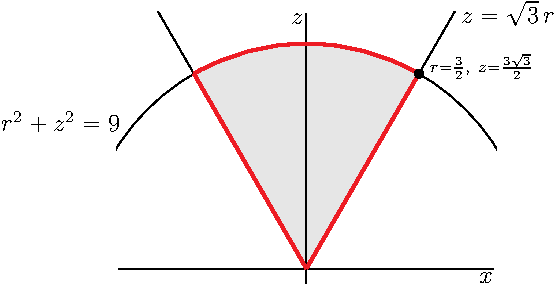
\includegraphics[scale=1.0]{fig/OE10A_8.pdf}
\end{center}
So
\begin{equation*}
T =\Set{(r\cos\theta\,,\,r\sin\theta\,,\,z)}{0\le r\le \tfrac{3}{2},\ 
                                             0\le\theta\le2\pi,\ 
                                          \sqrt{3}\,r\le z\le \sqrt{9-r^2}}
\end{equation*}
and
\begin{align*}
I &=\tripInt_V (x^2+y^2)\ \dee{V} 
   =\int_0^{3/2}\dee{r}\int_0^{2\pi}\dee{\theta}
           \int_{\sqrt{3}\,r}^{\sqrt{9-r^2}}\dee{z}\ 
                               r\overbrace{(r^2)}^{x^2+y^2}
   =\int_0^{3/2}\dee{r}\int_0^{2\pi}\dee{\theta}
                          \int_{\sqrt{3}\,r}^{\sqrt{9-r^2}}\dee{z}\ \ r^3
\end{align*}


(c) We'll use the spherical coordinate form.
\begin{align*}
I  &=\int_0^{3}\dee{\rho}\int_0^{2\pi}\dee{\theta}
           \int_0^{\pi/6}\dee{\varphi}\ \rho^4\sin^3\varphi \\
   &=\int_0^{3}\dee{\rho}\int_0^{2\pi}\dee{\theta}
           \int_0^{\pi/6}\dee{\varphi}\ \rho^4\sin\varphi
              \big[1-\cos^2\varphi\big] \\
   &=2\pi \int_0^3\dee{\rho}\ \rho^4
                \left[-\cos\varphi +\frac{\cos^3\varphi}{3}\right]_0^{\pi/6}
    =2\pi \left[-\frac{\sqrt{3}}{2} + \frac{\sqrt{3}}{8}+1-\frac{1}{3}\right]
                      \int_0^3\dee{\rho}\ \rho^4 \\
    &=2\pi \frac{3^5}{5}\left[\frac{2}{3} - \frac{3\sqrt{3}}{8}\right]
     =\overbrace{81}^{3^4}\pi \left[\frac{4}{5} - \frac{9\sqrt{3}}{20}\right]
     \approx 5.24
% 5.236243474
% 1.666748 \pi
\end{align*}
\end{solution}

%%%%%%%%%%%%%%%%%%%%%%%%%%%%%%%%
\begin{question}[M200 2011A] %8
Let $E$ be the ``ice cream cone'' $x^2 + y^2 + z^2 \le 1$, 
$x^2 + y^2 \le z^2$ , $z \ge 0$. Consider
\begin{equation*}
J =\tripInt_E \sqrt{x^2+y^2+z^2}\ \dee{V}
\end{equation*}
\begin{enumerate}[(a)]
\item
Write $J$ as an iterated integral, with limits, in cylindrical coordinates.
\item
Write $J$ as an iterated integral, with limits, in spherical coordinates.
\item
Evaluate $J$.
\end{enumerate}
\end{question}

%\begin{hint}
%
%\end{hint}

\begin{answer}
(a) $\int_0^{1/\sqrt{2}}\dee{r}\int_0^{2\pi}\dee{\theta}
           \int_r^{\sqrt{1-r^2}}\dee{z}\ r\sqrt{r^2+z^2}$

(b) $\int_0^{1}\dee{\rho}\int_0^{2\pi}\dee{\theta}
           \int_0^{\pi/4}\dee{\varphi}\ \rho^3\sin\varphi$

(c) $\frac{\pi}{2}\ \left[1-\frac{1}{\sqrt{2}}\right]$
\end{answer}

\begin{solution}
(a)
In cylindrical coordinates
\begin{itemize}
\item
$x^2+y^2+z^2\le 1$ is $r^2+z^2\le 1$ and
\item
$x^2+y^2\le z^2$ is $r^2\le z^2$ and
\item
$\dee{V}$ is $r\,\dee{r}\,\dee{\theta}\,\dee{z}$
\end{itemize}
Observe that $r^2+z^2= 1$ and $r^2= z^2$ intersect when $r^2=z^2=\frac{1}{2}$.
Here is a sketch of the $y=0$ cross--section of $E$.
\begin{center}
     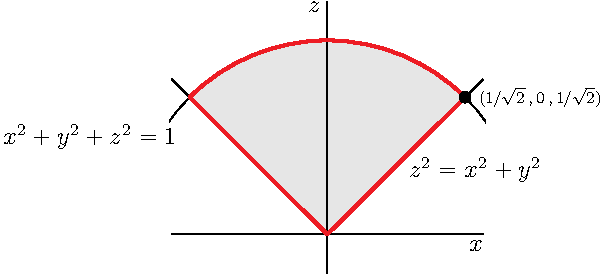
\includegraphics[scale=1.0]{fig/OE11A_8.pdf}
\end{center}
So
\begin{equation*}
E =\Set{(r\cos\theta\,,\,r\sin\theta\,,\,z)}{0\le r\le\nicefrac{1}{\sqrt{2}},\ 
                                             0\le\theta\le2\pi,\ 
                                              r\le z\le \sqrt{1-r^2}}
\end{equation*}
and
\begin{align*}
J &=\tripInt_E \sqrt{x^2+y^2+z^2}\ \dee{V} 
   =\int_0^{1/\sqrt{2}}\dee{r}\int_0^{2\pi}\dee{\theta}
           \int_r^{\sqrt{1-r^2}}\dee{z}\ r\sqrt{r^2+z^2}
\end{align*}

(b)
In spherical coordinates
\begin{itemize}
\item
$x^2+y^2+z^2\le 1$ is $\rho\le 1$ and
\item
$x^2+y^2\le z^2$ is $\rho^2\sin^2\varphi\le \rho^2\cos^2\varphi$,
or $\tan\varphi\le 1$ or $\varphi\le\frac{\pi}{4}$, and
\item
$\dee{V}$ is $\rho^2\sin\varphi\,\dee{\rho}\,\dee{\theta}\,\dee{\varphi}$
\end{itemize}
So
\begin{equation*}
E =\Set{(\rho\sin\varphi\cos\theta\,,\,\rho\sin\varphi\sin\theta\,,\,
          \rho\cos\varphi)}{0\le\rho\le 1,\  0\le\theta\le2\pi,\ 
                            0\le \varphi\le \nicefrac{\pi}{4}}
\end{equation*}
and, since the integrand $\sqrt{x^2+y^2+z^2}=\rho$,
\begin{align*}
J &=\tripInt_E \sqrt{x^2+y^2+z^2}\ \dee{V} 
   =\int_0^{1}\dee{\rho}\int_0^{2\pi}\dee{\theta}
           \int_0^{\pi/4}\dee{\varphi}\ \rho^2\sin\varphi\ \rho \\
   &=\int_0^{1}\dee{\rho}\int_0^{2\pi}\dee{\theta}
           \int_0^{\pi/4}\dee{\varphi}\ \rho^3\sin\varphi
\end{align*}


(c) We'll use the spherical coordinate form to evaluate
\begin{align*}
J &=\int_0^{1}\dee{\rho}\int_0^{2\pi}\dee{\theta}
           \int_0^{\pi/4}\dee{\varphi}\ \rho^3\sin\varphi \\
   &=2\pi \int_0^{1}\dee{\rho}\ \rho^3
                     \Big[-\cos\varphi\Big]_0^{\pi/4} 
    =2\pi\ \frac{1}{4}\ \left[1-\frac{1}{\sqrt{2}}\right] \\
    &=\frac{\pi}{2}\ \left[1-\frac{1}{\sqrt{2}}\right]
\end{align*}
\end{solution}

%%%%%%%%%%%%%%%%%%%%%%%%%%%%%%%%
\begin{question}[M200 2011D] %8
The body of a snowman is formed by the snowballs $x^2 + y^2 + z^2 = 12$ 
(this is its body) and $x^2 + y^2 + (z - 4)^2 = 4$ (this is its head).
\begin{enumerate}[(a)]
\item
Find the volume of the snowman by subtracting the intersection of the two snow
balls from the sum of the volumes of the snow balls. [Recall that the volume of a
sphere of radius $r$ is $\frac{4\pi}{3} r^3$.]

\item
We can also calculate the volume of the snowman as a sum of the following triple integrals:
\begin{enumerate}[1.]
\item
\begin{equation*}
\int_0^{\frac{2\pi}{3}} \int_0^{2\pi}  \int_0^2 \rho^2\sin{\varphi}
                 \  \dee{\rho}\,\dee{\theta}\,\dee{\varphi}
\end{equation*}
\item
\begin{equation*}
\int_0^{2\pi} \int_0^{\sqrt{3}}  \int_{\sqrt{3}\,r}^{4-\frac{r}{\sqrt{3}}}
                            r\ \dee{z}\,\dee{r}\,\dee{\theta}
\end{equation*}
\item
\begin{equation*}
\int_{\frac{\pi}{6}}^\pi  \int_0^{2\pi} \int_0^{2\sqrt{3}}
                \rho^2\sin(\varphi)\ \dee{\rho}\,\dee{\theta}\,\dee{\varphi}
\end{equation*}
\end{enumerate}
Circle the right answer from the underlined choices and fill in the blanks 
in the following descriptions of the region of integration for each integral. 
[Note: We have translated the axes in order to write down some of the 
integrals above. The equations you specify should be those before 
the translation is performed.]
\begin{enumerate}[i.]
\item
The region of integration in (1) is a part of the snowman's 
\begin{align*}
    &\text{\underline{body/head/body and head}.}
\intertext{It is the solid enclosed by the}
    &\text{\underline{sphere/cone} defined by the equation  
                     $\rule{1.2in}{0.15mm}$}\\
\intertext{and the}
    &\text{\underline{sphere/cone} defined by the equation
$\rule{1.5in}{0.15mm}$.}
\end{align*}
\item
The region of integration in (2) is a part of the snowman's 
\begin{align*}
    &\text{\underline{body/head/body and head}.}
\intertext{It is the solid enclosed by the}
    &\text{\underline{sphere/cone} defined by the equation  
                       $\rule{1.2in}{0.15mm}$}
\intertext{and the}
    &\text{\underline{sphere/cone} defined by the equation
                 $\rule{1.5in}{0.15mm}$.}
\end{align*}
\item
The region of integration in (3) is a part of the snowman's 
\begin{align*}
    &\text{\underline{body/head/body and head}.}
\intertext{It is the solid enclosed by the}
    &\text{\underline{sphere/cone} defined by the equation
                    $\rule{1.2in}{0.15mm}$}
\intertext{and the}
     &\text{\underline{sphere/cone} defined by the equation
                $\rule{1.5in}{0.15mm}$.}
\end{align*}
\end{enumerate}
\end{enumerate}
\end{question}

%\begin{hint}
%
%\end{hint}

\begin{answer}
(a) $\frac{2\pi}{3}\left[\big(12\big)^{3/2}+54\right]$

(b) i. The top part is the part of the snowman's head that is inside the sphere\\
$
x^2+y^2+(z-4)^2 = 4
$
and above the cone
$
z-4 = - \sqrt{\frac{x^2+y^2}{3}}
$.

ii. The middle part is the part of the snowman's head and body that 
is bounded on the top by the  cone
$
z-4 = - \sqrt{\frac{x^2+y^2}{3}}
$
and is bounded on the bottom by the cone
$
z = \sqrt{3(x^2+y^2)}
$.

iii. The bottom part is the part of the snowman's body that is inside 
the sphere\\
$
x^2+y^2+z^2 = 12
$
and is below the cone
$
z = \sqrt{3(x^2+y^2)}
$.
\end{answer}

\begin{solution}
(a) 
As a check, the body of the snow man has radius $\sqrt{12} = 2\sqrt{3}
\approx 3.46$, which is between $2$ (the low point of the head) and $4$
(the center of the head). Here is a sketch of a side view of the snowman.
\begin{center}
     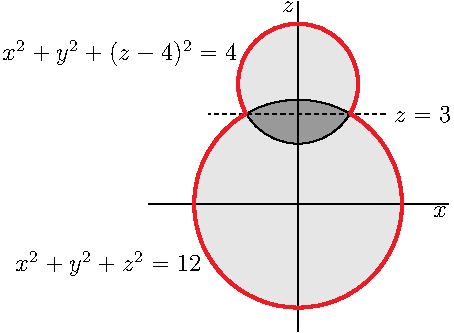
\includegraphics{fig/OE11D_8a.pdf}
\end{center}
We want to determine the volume of the intersection of the body and the head,
whose side view is the darker shaded region in the sketch.
\begin{itemize}
\item
The outer boundary of the body and the outer boundary of the head 
intersect when both $x^2 + y^2 + z^2 = 12$ and $x^2 + y^2 + (z - 4)^2 = 4$.
Subtracting the second equation from the first gives
\begin{equation*}
z^2-(z-4)^2 =12 -4
\iff
8z-16 =8
\iff
z=3
\end{equation*}
Then substituting $z=3$ into either equation gives $x^2+y^2=3$.
So the intersection of the outer boundaries of the head and body 
(i.e. the neck)
is the circle $x^2+y^2=3$, $z=3$.
\item
The top boundary of the intersection is part of the top half
of the snowman's body and so has equation $z=+\sqrt{12-x^2-y^2}$.
\item
The bottom boundary of the intersection is part of the bottom half of the snowman's head, and so has equation $z=4-\sqrt{4-x^2-y^2}$
\end{itemize}
The intersection of the head and body is thus
\begin{align*}
\cV = \Set{(x,y,z}{x^2+y^2\le 3,\ 
            4-\sqrt{4-x^2-y^2}\le z\le \sqrt{12-x^2-y^2}}
\end{align*}
We'll compute the volume of $\cV$ using cylindrical coordinates
\begin{align*}
\text{Volume}(\cV) &= \int_0^{\sqrt{3}}\dee{r}\int_0^{2\pi}\dee{\theta}
                     \int_{4-\sqrt{4-r^2}}^{\sqrt{12-r^2}}\dee{z}\ r \\
   &=\int_0^{\sqrt{3}}\dee{r}\ 2\pi\ r\big[\sqrt{12-r^2}-4+\sqrt{4-r^2}\big] \\
   &=2\pi\left[-\frac{1}{3}{\big(12-r^2\big)}^{3/2}
               -2r^2
               -\frac{1}{3}{\big(4-r^2\big)}^{3/2}\right]_0^{\sqrt{3}} \\
   &= 2\pi\left[-\frac{1}{3}{\big(9\big)}^{3/2}
               -2(3)
               -\frac{1}{3}{\big(1\big)}^{3/2}
               +\frac{1}{3}{\big(12\big)}^{3/2}
               +2(0)^2
               +\frac{1}{3}{\big(4\big)}^{3/2}
               \right] \displaybreak[0]\\
   &= 2\pi\left[-9
               -6
               -\frac{1}{3}
               +\frac{1}{3}{\big(12\big)}^{3/2}
               +\frac{8}{3}
               \right] \\
   &=2\pi\left[\frac{1}{3}{\big(12\big)}^{3/2}
               -\frac{38}{3}
               \right]
\end{align*}
So the volume of the snowman is
\begin{align*}
&\frac{4\pi}{3}\big(12\big)^{3/2}
+\frac{4\pi}{3} 2^3
-2\pi\left[\frac{1}{3}{\big(12\big)}^{3/2}
               -\frac{38}{3}
               \right] \\
&\hskip0.5in=\frac{2\pi}{3}\left[\big(12\big)^{3/2}+54\right]
\end{align*}

(b) The figure on the left below is another side view of the snowman.
This time it is divided into a lighter gray top part, a darker gray
middle part and a lighter gray bottom part. The figure on the
right below is an enlarged view of the central part of the figure on the
left.
\begin{center}
     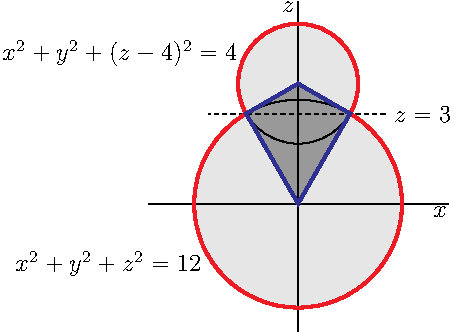
\includegraphics{fig/OE11D_8b.pdf}\qquad
     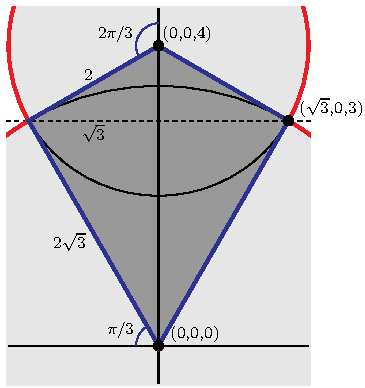
\includegraphics{fig/OE11D_8c.pdf}
\end{center}

i. The top part is the Pac--Man
\begin{center}
     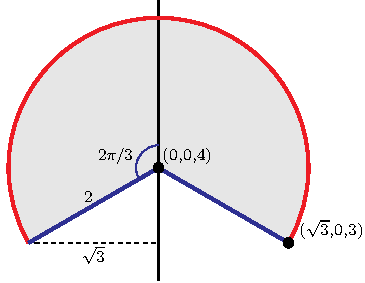
\includegraphics{fig/OE11D_8d.pdf}
\end{center}
part of the snowman's head. It is the part of the sphere
\begin{equation*}
x^2+y^2+(z-4)^2\le 4
\end{equation*}
that is above the cone
\begin{equation*}
z-4 = - \sqrt{\frac{x^2+y^2}{3}}
\end{equation*}
(which contains the points $(0,0,4)$ and $(\sqrt{3},0,3)$).

ii. The middle part is the diamond shaped
\begin{center}
     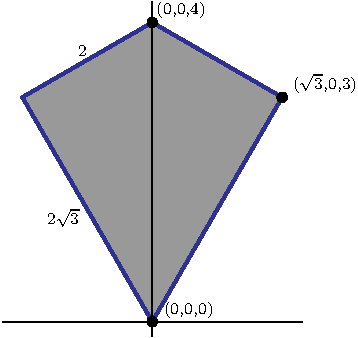
\includegraphics{fig/OE11D_8e.pdf}
\end{center}
part of the snowman's head and body. It is bounded on the top by the  cone
\begin{equation*}
z-4 = - \sqrt{\frac{x^2+y^2}{3}}
\end{equation*}
(which contains the points $(0,0,4)$ and $(\sqrt{3},0,3)$) and
is bounded on the bottom by the  cone
\begin{equation*}
z = \sqrt{3(x^2+y^2)}
\end{equation*}
(which contains the points $(0,0,0)$ and $(\sqrt{3},0,3)$).

iii. The bottom part is the Pac--Man
\begin{center}
     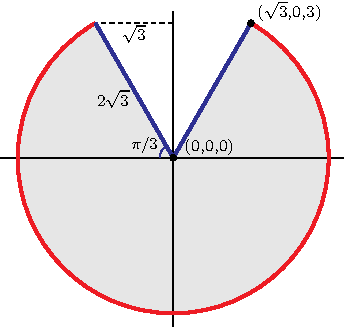
\includegraphics{fig/OE11D_8f.pdf}
\end{center}
part of the snowman's body. It is the part of the sphere
\begin{equation*}
x^2+y^2+z^2\le 12
\end{equation*}
that is below the cone
\begin{equation*}
z = \sqrt{3(x^2+y^2)}
\end{equation*}
(which contains the points $(0,0,0)$ and $(\sqrt{3},0,3)$).
\end{solution}

\begin{question}[M200 2013D] %9
\begin{enumerate}[(a)]
\item
Find the volume of the solid inside the surface defined by the equation 
$\rho = 8 \sin(\varphi)$ in spherical coordinates.

You may use that
\begin{equation*}
\int \sin^4(\varphi) =\frac{1}{32}\big(12\varphi -8\sin(2\varphi)
+\sin(4\varphi)\big) +C
\end{equation*}

\item
Sketch this solid or describe what it looks like. 
\end{enumerate}
\end{question}

\begin{hint}
(b) it is a solid of revolution.
\end{hint}

\begin{answer}
(a) $\frac{2(8^3)\,\pi}{3}\ \frac{12\,\pi}{32}=128\pi^2$

(b) The surface is a torus (a donut) but with the hole in the centre 
shrunk to a point.
The figure below is a sketch of the part of the surface in the
first octant.

\begin{center}
     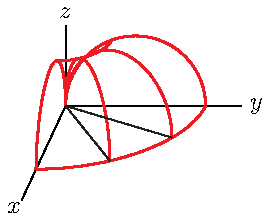
\includegraphics{fig/torusB.pdf}
\end{center}
\end{answer}

\begin{solution}
(a)
Recall that, in spherical coordinates, $\varphi$ runs from $0$ (that's the
positive $z$--axis) to $\pi$ (that's the negative $z$--axis),
$\theta$ runs from $0$ to $2\pi$ ($\theta$ is the regular polar 
or cylindrical coordinate)
and 
 $\dee{V} = \rho^2\ \sin\varphi\ \dee{\rho}\,\dee{\theta}\,\dee{\varphi}$.
So
\begin{align*}
\text{Volume} & = \int_0^\pi \dee{\varphi}\int_0^{2\pi}\dee{\theta}
                      \int_0^{8\sin\varphi}\dee{\rho}\ \rho^2\ \sin\varphi \\
& = \int_0^\pi \dee{\varphi}\int_0^{2\pi}\dee{\theta}\ 
                      \frac{(8\sin\varphi)^3}{3} \sin\varphi \\
& = \frac{2(8^3)\,\pi}{3} \int_0^\pi \dee{\varphi}\ 
                       \sin^4\varphi \\
&= \frac{2(8^3)\,\pi}{3} \left[\frac{1}{32}\big(12\varphi -8\sin(2\varphi)
+\sin(4\varphi)\big)\right]_0^\pi \\
&=\frac{2(8^3)\,\pi}{3}\ \frac{12\,\pi}{32}
=128\pi^2
\end{align*}

(b) Fix any $\varphi$ between $0$ and $\pi$. If $\rho=8\sin\varphi$,
then as $\theta$ runs from $0$ to $2\pi$,
\begin{align*}
(x,y,z) &= \big(\rho\sin\varphi\cos\theta\,,\,\rho\sin\varphi\sin\theta\,,\,
               \rho\cos\varphi\big) \\
        &= \big(8\sin^2\varphi\cos\theta\,,\,8\sin^2\varphi\sin\theta\,,\,
               8\sin\varphi\cos\varphi\big) \\
        &= \big(R\cos\theta\,,\,R\sin\theta\,,\,Z\big)\qquad
        \text{with }R=8\sin^2\varphi,\ Z= 8\sin\varphi\cos\varphi
\end{align*}
sweeps out a circle of radius $R=8\sin^2\varphi$ contained in the plane 
$z=Z=8\sin\varphi\cos\varphi$ and centred on
$\big(0,0,Z=8\sin\varphi\cos\varphi\big)$. So the surface is
a bunch of circles stacked one on top of the other. It is a surface of
revolution. We can sketch it by 
\begin{itemize}
\item 
first sketching the $\theta=0$ section of the surface (that's the part of
the surface in the right half of the $xz$--plane)
\item
and then rotate the result about the $z$--axis.
\end{itemize}
The $\theta=0$ part of the surface is
\begin{align*}
&\Set{(x,y,z)}{x=8\sin^2\varphi,\ y=0,\ z=8\sin\varphi\cos\varphi,\ 
                     0\le\varphi\le \pi} \\
&=\Set{(x,y,z)}{x=4-4\cos(2\varphi),\ y=0,\ z=4\sin(2\varphi),\ 
                     0\le\varphi\le \pi}
\end{align*}
It's a circle of radius $4$, contained in the $xz$--plane (i.e. $y=0$)
and centred on $(4,0,0)$! The figure on the left below is a sketch of the
top half of the circle. When we rotate the circle about the $z$--axis
we get a torus (a donut) but with the hole in the centre shrunk to a point.
The figure on the right below is a sketch of the part of the torus in the
first octant.

\begin{center}
     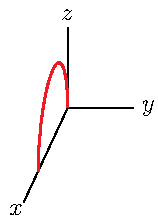
\includegraphics{fig/torusA.pdf}\qquad
     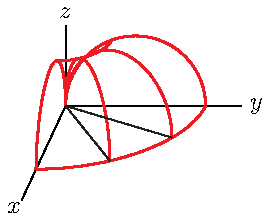
\includegraphics{fig/torusB.pdf}
\end{center}
\end{solution}

\begin{question}[M200 2014A] %8
Let $E$ be the solid
\begin{equation*}
0 \le z \le \sqrt{x^2 + y^2},\qquad
x^2 + y^2 \le 1,
\end{equation*}
and consider the integral
\begin{equation*}
I = \tripInt_E z \sqrt{x^2 + y^2 + z^2}\  \dee{V}.
\end{equation*}
\begin{enumerate}[(a)]
\item
Write the integral $I$ in cylindrical coordinates.

\item
Write the integral $I$ in spherical coordinates.

\item
Evaluate the integral $I$ using either form.
\end{enumerate}
\end{question}

%\begin{hint}
%
%\end{hint}

\begin{answer}
(a) $I = \int_0^1\dee{r} \int_0^{2\pi}\dee{\theta} \int_0^r\dee{z}\ 
           r\ z\ \sqrt{r^2+z^2}$\qquad
(b) $I = \int_{\pi/4}^{\pi/2}\dee{\varphi} 
                \int_0^{2\pi}\dee{\theta} 
                \int_0^{1/\sin\varphi}\dee{\rho}\ 
                \rho^4\sin\varphi \ \cos\varphi$ 

(c) $\frac{2(2\sqrt{2}-1)\pi}{15}$
\end{answer}

\begin{solution}
(a) In cylindrical coordinates $0\le z\le \sqrt{x^2+y^2}$ becomes
$0\le z\le r$, and $x^2+y^2\le 1$ becomes $0\le r\le 1$. So
\begin{equation*}
E = \Set{(r\cos\theta\,,\,r\sin\theta\,,\,z)}{0\le r\le 1,\ 0\le\theta\le 2\pi,
              \ 0\le z\le r}
\end{equation*}
and, since $\dee{V} = r\,\dee{r}\,\dee{\theta}\,\dee{z}$,
\begin{align*}
I &= \tripInt_E z \sqrt{x^2 + y^2 + z^2}\  \dee{V} 
  = \int_0^1\dee{r} \int_0^{2\pi}\dee{\theta} \int_0^r\dee{z}\ 
           r\ z\ \sqrt{\underbrace{r^2+z^2}_{x^2+y^2+z^2}}
\end{align*} 

(b)
Here is a sketch of a constant $\theta$ section of $E$.

\begin{center}
     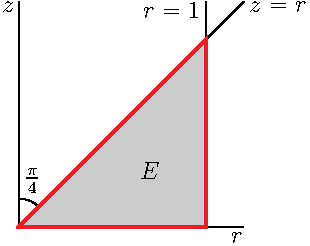
\includegraphics{fig/OE14A_8.pdf}
\end{center}

Recall that the spherical coordinate $\varphi$ is the angle
between the $z$--axis and the radius vector. 
So, in spherical coordinates $z=r$ (which makes an angle $\frac{\pi}{4}$
with the $z$ axis) becomes $\varphi=\frac{\pi}{4}$, and
the plane $z=0$, i.e. the $xy$--plane, becomes $\varphi=\frac{\pi}{2}$,
and $r=1$ becomes $\rho\sin\varphi = 1$.  So
\begin{equation*}
E = \left\{(\rho\sin\varphi\cos\theta\,,\,\rho\sin\varphi\sin\theta\,,\,
          \rho\cos\varphi)\ \left|\ 
                    \frac{\pi}{4}\le \varphi\le \frac{\pi}{2},
            \ 0\le\theta\le 2\pi,
              \ 0\le \rho\le \frac{1}{\sin\varphi}\ \right.\right\}
\end{equation*}
and, since 
  $\dee{V} = \rho^2\sin\varphi\,\dee{\rho}\,\dee{\theta}\,\dee{\varphi}$,
\begin{align*}
I &= \tripInt_E z \sqrt{x^2 + y^2 + z^2}\  \dee{V}
  = \int_{\pi/4}^{\pi/2}\dee{\varphi} 
                \int_0^{2\pi}\dee{\theta} 
                \int_0^{1/\sin\varphi}\dee{\rho}\ 
                \rho^2\sin\varphi \ 
           \overbrace{\rho\cos\varphi}^{z}\ \rho \\
  &= \int_{\pi/4}^{\pi/2}\dee{\varphi} 
                \int_0^{2\pi}\dee{\theta} 
                \int_0^{1/\sin\varphi}\dee{\rho}\ 
                \rho^4\sin\varphi \ \cos\varphi
\end{align*} 

(c) We'll integrate using the spherical coordinate version.
\begin{align*}
I &= \int_{\pi/4}^{\pi/2}\dee{\varphi} 
                \int_0^{2\pi}\dee{\theta} 
                \int_0^{1/\sin\varphi}\dee{\rho}\ 
                \rho^4\sin\varphi \ \cos\varphi \\
  &= \int_{\pi/4}^{\pi/2}\dee{\varphi} 
                \int_0^{2\pi}\dee{\theta}\ 
                \frac{1}{5\sin^5\varphi}\sin\varphi \ \cos\varphi \\
  &= \frac{2\pi}{5}\int_{\pi/4}^{\pi/2}\dee{\varphi}\ 
                \frac{\cos\varphi}{\sin^4\varphi} \\
  &= \frac{2\pi}{5}\int_{1/\sqrt{2}}^{1} 
                \frac{\dee{u}}{u^4}\qquad\text{with }
                     u=\sin\varphi,\ \dee{u}=\cos\varphi\,\dee{\varphi} \\
  &= \frac{2\pi}{5} \left[\frac{u^{-3}}{-3}\right]_{1/\sqrt{2}}^{1}  \\
  &= \frac{2(2\sqrt{2}-1)\pi}{15}
\end{align*} 
\end{solution}

\begin{question}[M200 2014D] %8
Consider the iterated integral
\begin{equation*}
I =\int_{-a}^0\int_{-\sqrt{a^2-x^2}}^0 \int_0^{\sqrt{a^2-x^2-y^2}}
    \big(x^2+y^2+z^2\big)^{2014}\ \dee{z}\,\dee{y}\,\dee{x}
\end{equation*}
where $a$ is a positive constant.
\begin{enumerate}[(a)]
\item
Write $I$ as an iterated integral in cylindrical coordinates.
\item
Write $I$ as an iterated integral in spherical coordinates.
\item
Evaluate I using whatever method you prefer.
\end{enumerate}
\end{question}

%\begin{hint}
%
%\end{hint}

\begin{answer}
(a) $\int_0^a \dee{z}\int_{\pi}^{3\pi/2}\dee{\theta} 
      \int_0^{\sqrt{a^2-z^2}}\dee{r}\ r\big(r^2+z^2\big)^{2014}$\qquad
(b) $\int_0^{\pi/2} \dee{\varphi}\int_{\pi}^{3\pi/2}\dee{\theta} 
     \int_0^a\dee{\rho}\ \rho^{4030}\sin\varphi$

(c) $\frac{a^{4031}\pi}{8062}$
\end{answer}

\begin{solution}
The main step is to figure out what the domain of integration 
looks like. 
\begin{itemize}
\item
The outside integral says that $x$ runs from $-a$ to $0$. 
\item
The middle integrals says that, for each $x$ in that range, $y$ runs
from $-\sqrt{a^2-x^2}$ to $0$. We can rewrite $y=-\sqrt{a^2-x^2}$
in the more familiar form $x^2+y^2=a^2$, $y\le 0$. So $(x,y)$
runs over the third quadrant part of the disk of radius $a$, centred 
on the origin.

\begin{center}
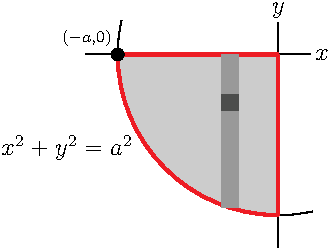
\includegraphics{fig/OE14D_8AA.pdf}
\end{center}

\item
Finally, the inside integral says that, for each $(x,y)$ in the quarter disk,
$z$ runs from $0$ to $\sqrt{a^2-x^2-y^2} $. We can also rewrite
$z=\sqrt{a^2-x^2-y^2}$ in the more familiar form $x^2+y^2+z^2=a^2$, $z\ge 0$.
\end{itemize}
So the domain of integration is the part of the interior of the sphere
of radius $a$, centred on the origin, that lies in the octant
$x\le 0$, $y\le 0$, $z\ge 0$.
\begin{align*}
V&=\Set{(x,y,z)}{-a\le x\le 0,\ -\sqrt{a^2-x^2}\le y\le 0,\ 
                 0\le z\le\sqrt{a^2-x^2-y^2} } \\
&=\Set{(x,y,z)}{x^2+y^2+z^2\le a^2,\ x\le 0,\ y\le 0,\ z\ge 0 }
\end{align*}

\begin{center}
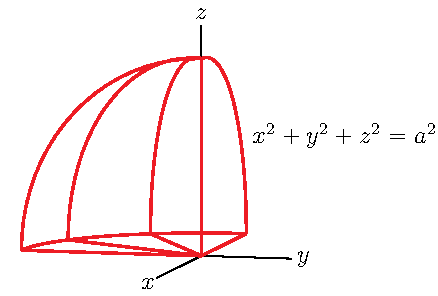
\includegraphics[scale=0.95]{fig/OE14D_8BB.pdf}
\end{center}


(a) Note that, in $V$, $(x,y)$ is restricted to the third
quadrant, which in cylindrical coordinates 
is $\pi\le\theta\le\frac{3\pi}{2}$. So, in cylindrical coordinates,
\begin{align*}
V&=\Big\{(r\cos\theta,r\sin\theta,z)\ \Big|\ 
          r^2+z^2\le a^2,\ \pi\le\theta\le\frac{3\pi}{2},\ z\ge 0 \Big\} \\
 &=\Big\{(r\cos\theta,r\sin\theta,z)\ \Big|\ 0\le z\le a,\ 
          \pi\le\theta\le\frac{3\pi}{2},\ 0\le r\le\sqrt{a^2-z^2} \Big\}
\end{align*}
and
\begin{align*}
I&= \tripInt_V \big(x^2+y^2+z^2\big)^{2014}\ \dee{V}
  = \tripInt_V \big(r^2+z^2\big)^{2014}\ r\,\dee{r}\,\dee{\theta}\,\dee{z} \\
&=\int_0^a \dee{z}\int_{\pi}^{3\pi/2}\dee{\theta} 
     \int_0^{\sqrt{a^2-z^2}}\dee{r}\ r\big(r^2+z^2\big)^{2014}
\end{align*}

(b) The spherical coordinate $\varphi$ runs from $0$ (when the radius
vector is along the positive $z$--axis)  to $\nicefrac{\pi}{2}$
(when the radius vector lies in the $xy$--plane) so that
\begin{align*}
I&= \tripInt_V \big(x^2+y^2+z^2\big)^{2014}\ \dee{V}
  = \tripInt_V \rho^{2\times 2014}\ \rho^2\sin\varphi\ 
                 \dee{\rho}\,\dee{\theta}\,\dee{\varphi} \\
&=\int_0^{\pi/2} \dee{\varphi}\int_{\pi}^{3\pi/2}\dee{\theta} 
     \int_0^a\dee{\rho}\ \rho^{4030}\sin\varphi
\end{align*}

(c) Using the spherical coordinate version
\begin{align*}
I&=\int_0^{\pi/2} \dee{\varphi}\int_{\pi}^{3\pi/2}\dee{\theta} 
     \int_0^a\dee{\rho}\ \rho^{4030}\sin\varphi \\
 &=\frac{a^{4031}}{4031}
      \int_0^{\pi/2} \dee{\varphi}\int_{\pi}^{3\pi/2}\dee{\theta} 
          \ \sin\varphi \\
 &=\frac{a^{4031}\pi}{8062}
      \int_0^{\pi/2} \dee{\varphi}\ \sin\varphi \\
 &=\frac{a^{4031}\pi}{8062}
\end{align*}
\end{solution}

%%%%%%%%%%%%%%%%%%%%%%%%%%%%%%%%
\begin{question}[M200 2015D] %8
The solid $E$ is bounded below by the paraboloid $z = x^2 + y^2$ 
and above by the cone $z=\sqrt{x^2+y^2}$. Let
\begin{equation*}
I = \tripInt_E z\big(x^2+y^2+z^2\big)\ \dee{V}
\end{equation*}
\begin{enumerate}[(a)]
\item
Write $I$ in terms of cylindrical coordinates. Do not evaluate.
\item
Write $I$ in terms of spherical coordinates. Do not evaluate.
\item
Calculate $I$.
\end{enumerate}
\end{question}

%\begin{hint}
%
%\end{hint}

\begin{answer}
(a) $\int_0^1 \dee{r}\ r \int_0^{2\pi}\dee{\theta} \int_{r^2}^r\dee{z}\
           z(r^2+z^2)$\qquad
(b) $\int_{\pi/4}^{\pi/2} \dee{\varphi} \int_0^{2\pi}\dee{\theta}
         \int_0^{\cos\varphi/\sin^2\varphi} \dee{\rho}\ \rho^5\sin\varphi 
             \cos\varphi$

(c) $\frac{3\pi}{40}$
\end{answer}

\begin{solution}
(a)
In cylindrical coordinates, the paraboloid is $z=r^2$ and
the cone is $z=r$. The two meet when $r^2=r$. That is, when $r=0$
and when $r=1$. So, in cylindrical coordinates
\begin{align*}
I = \int_0^1 \dee{r}\ r \int_0^{2\pi}\dee{\theta} \int_{r^2}^r\dee{z}\
           z(r^2+z^2)
\end{align*}

(b) In spherical coordinates, the paraboloid is 
\begin{equation*}
\rho\cos\varphi=\rho^2\sin^2\varphi\qquad\text{or}\qquad
     \rho=\frac{\cos\varphi}{\sin^2\varphi}
\end{equation*}
and the cone is 
\begin{equation*}
\rho\cos\varphi=\rho\sin\varphi\quad\text{or}\quad
\tan\varphi=1\quad\text{or}\quad
\varphi=\frac{\pi}{4}
\end{equation*} 
The figure below shows  a constant $\theta$ cross--section of
$E$. Looking at that figure, we see that $\varphi$ runs from
$\frac{\pi}{4}$ (i.e. the cone) to $\frac{\pi}{2}$
(i.e. the $xy$--plane).

\begin{center}
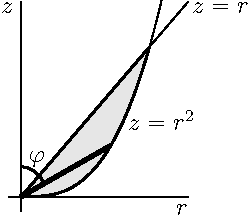
\includegraphics{fig/OE15D_8.pdf}
\end{center}

So, is spherical coordinates,
\begin{align*}
I &= \int_{\pi/4}^{\pi/2} \dee{\varphi} \int_0^{2\pi}\dee{\theta}
         \int_0^{\cos\varphi/\sin^2\varphi} \dee{\rho}\ \rho^2\sin\varphi \ 
             \overbrace{\rho\cos\varphi}^{z}
             \overbrace{\rho^2}^{x^2+y^2+z^2} \\
&= \int_{\pi/4}^{\pi/2} \dee{\varphi} \int_0^{2\pi}\dee{\theta}
         \int_0^{\cos\varphi/\sin^2\varphi} \dee{\rho}\ \rho^5\sin\varphi 
             \cos\varphi
\end{align*}

(c) The cylindrical coordinates integral looks easier.
\begin{align*}
I &= \int_0^1 \dee{r}\ r \int_0^{2\pi}\dee{\theta} \int_{r^2}^r\dee{z}\
           z(r^2+z^2) \\
  &= \int_0^1 \dee{r}\ r \int_0^{2\pi}\dee{\theta}\ 
               \left[r^2\frac{z^2}{2}+\frac{z^4}{4}\right]_{r^2}^r \\
  &= 2\pi \int_0^1 \dee{r}\ r  
               \left[r^2\frac{r^2}{2}+\frac{r^4}{4}
               -r^2\frac{r^4}{2}-\frac{r^8}{4}\right] \\
  &=2\pi \left[\frac{1}{12}+\frac{1}{24}
               -\frac{1}{16}-\frac{1}{40}\right]
   =\frac{\pi}{2} \left[\frac{1}{3}+\frac{1}{6}
               -\frac{1}{4}-\frac{1}{10}\right] \\
   &=\frac{3\pi}{40}
\end{align*}
\end{solution}

%%%%%%%%%%%%%%%%%%%%%%%%%%%%%%%%
\begin{question}[M200 2016D] %7
Let $S$ be the region on the first octant (so that $x,y,z\ge 0$)
which lies above the cone $z=\sqrt{x^2+y^2}$ and below the sphere
$(z-1)^2 +x^2+y^2=1$. Let $V$ be its volume.
\begin{enumerate}[(a)]
\item
Express $V$ as a triple integral in cylindrical coordinates.
\item
Express $V$ as an triple integral in spherical coordinates.
\item
Calculate $V$ using either of the integrals above.
\end{enumerate}
\end{question}

%\begin{hint}
%
%\end{hint}

\begin{answer}
(a) 
$V  = \int_0^1\dee{r} \int_0^{\pi/2}\dee{\theta}\int_r^{1+\sqrt{1-r^2}}\dee{z}
     \ r$\qquad
(b)
$V = \int_0^{\pi/4}\dee{\varphi} \int_0^{\pi/2}\dee{\theta}
               \int_0^{2\cos\varphi}\dee{\rho}\ \rho^2\sin\varphi$

(c) $\frac{\pi}{4}$
\end{answer}

\begin{solution}
Note that both the sphere $x^2+y^2+(z-1)^2=1$
and the cone $z=\sqrt{x^2+y^2}$  are invariant under rotations
around the $z$--axis. The sphere $x^2 + y^2 + (z-1)^2 = 1$ 
and the cone $z = \sqrt{x^2 + y^2}$ intersect when $z=\sqrt{x^2+y^2}$, so that
$x^2+y^2=z^2$, and
\begin{align*}
x^2 + y^2 + (z-1)^2 = z^2+(z-1)^2=1
&\iff 2z^2-2z=0
\iff 2z(z-1)=0 \\
&\iff z=0,1
\end{align*}
So the surfaces intersect on the circle $z=1$,
$x^2+y^2=1$ and
\begin{equation*}
S = \Set{(x,y,z)}{x,y\ge 0,\  x^2+y^2\le 1,\ 
         \sqrt{x^2+y^2}\le z\le 1+\sqrt{1-x^2-y^2}}
\end{equation*}
Here is a sketch of the $y=0$ cross section of S.
\begin{center}
     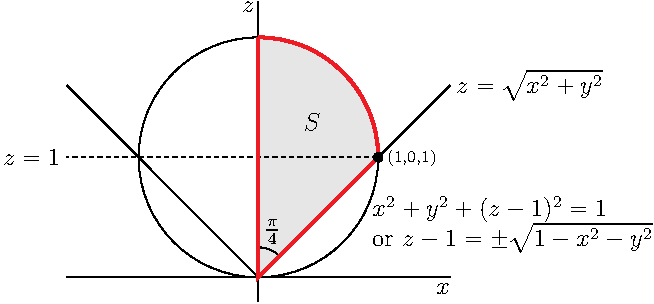
\includegraphics{fig/OE16D_7.pdf}
\end{center}

(a) In cylindrical coordinates
\begin{itemize}
\item
the condition $x,y\ge 0$ is $0\le\theta\le\nicefrac{\pi}{2}$,
\item
the condition $x^2+y^2\le 1$ is $r\le 1$, and
\item
the conditions $\sqrt{x^2+y^2}\le z\le 1+\sqrt{1-x^2-y^2}$
are $r\le z\le 1+\sqrt{1-r^2}$, and
\item
$\dee{V} = r\,\dee{r}\,\dee{\theta}\,\dee{z}$.
\end{itemize}
So
\begin{align*}
V = \tripInt_S\dee{V}
  = \int_0^1\dee{r} \int_0^{\pi/2}\dee{\theta}\int_r^{1+\sqrt{1-r^2}}\dee{z}
     \ r
\end{align*}

(b) In spherical coordinates, 
\begin{itemize}
\item 
the cone $z=\sqrt{x^2+y^2}$ becomes
\begin{align*}
\rho\,\cos\varphi =\sqrt{\rho^2\sin^2\varphi\,\cos^2\theta
                         +\rho^2\sin^2\varphi\,\sin^2\theta}
                  =\rho\sin\varphi
\iff \tan\varphi=1
\iff \varphi=\frac{\pi}{4}
\end{align*}
\item
so that, on $S$, the spherical coordinate $\varphi$ runs from $\varphi=0$
(the positive $z$ --axis) to $\varphi=\nicefrac{\pi}{4}$
(the cone $z=\sqrt{x^2+y^2}$), which keeps us above the cone,
\item
the condition $x,y\ge 0$ is $0\le\theta\le\nicefrac{\pi}{2}$,
\item
the condition $x^2+y^2+(z-1)^2\le 1$, (which keeps us inside the sphere),
becomes
\begin{align*}
&\rho^2\sin^2\varphi\,\cos^2\theta + \rho^2\sin^2\varphi\,\sin^2\theta
      +\big(\rho\cos\varphi-1\big)^2\le 1 \\
&\iff \rho^2\,\sin^2\varphi +\rho^2\cos^2\varphi -2\rho\cos\varphi +1  \le 1 \\
&\iff \rho^2-2\rho\cos\varphi\le 0 \\
&\iff \rho\le 2 \cos\varphi             
\end{align*}
\item
and $\dee{V} = \rho^2\sin\varphi\,\dee{\rho}\,\dee{\theta}\,\dee{\varphi}$.
\end{itemize}
So
\begin{align*}
V = \tripInt_S\dee{V}
  = \int_0^{\pi/4}\dee{\varphi} \int_0^{\pi/2}\dee{\theta}
               \int_0^{2\cos\varphi}\dee{\rho}\ \rho^2\sin\varphi 
\end{align*}

(c) We'll evaluate $V$ using the spherical coordinate integral of part (b).
\begin{align*}
V &= \int_0^{\pi/4}\dee{\varphi} \int_0^{\pi/2}\dee{\theta}
               \int_0^{2\cos\varphi}\dee{\rho}\ \rho^2\sin\varphi  \\
&=\frac{8}{3} \int_0^{\pi/4}\dee{\varphi} \int_0^{\pi/2}\dee{\theta}\ 
               \cos^3\varphi\ \sin\varphi \\
&=\frac{8}{3}\ \frac{\pi}{2}\ \left[-\frac{\cos^4\varphi}{4}\right]_0^{\pi/4} \\
&=\frac{\pi}{3} \left[1-\frac{1}{(\sqrt{2})^4}\right] \\
&=\frac{\pi}{4}
\end{align*}
\end{solution}

%%%%%%%%%%%%%%%%%%%%%%%%%%%%%%%%
\begin{question}[M200 2004A] %8
A solid is bounded below by the cone $z=\sqrt{3x^2+3y^2}$
and above by the sphere $x^2+y^2+z^2=9$. It has density $\de(x,y,z)=x^2+y^2$.
\begin{enumerate}[(a)]
\item
Express the mass $m$ of the solid as a triple integral in
cylindrical coordinates.
\item
Express the mass $m$ of the solid as a triple integral in
spherical coordinates.
\item 
Evaluate $m$.
\end{enumerate}
\end{question}

%\begin{hint}
%
%\end{hint}

\begin{answer}
(a) $\int_0^{2\pi}\dee{\theta}\int_0^{3/2}\dee{r}\ r\int_{\sqrt{3}\,r}^{\sqrt{9-r^2}}dz\ r^2$

(b) $\int_0^{2\pi}\dee{\theta}\int_0^{\pi/6}\dee{\varphi}\int_0^3\dee{\rho}\ \big(\rho^2\sin\varphi\big)
\big(\rho^2\sin^2\varphi\big)$

(c) $2\pi \frac{3^5}{5} \big[\frac{2}{3}-\frac{3\sqrt{3}}{8}\big]$
\end{answer}

\begin{solution}
(a) 
In cylindrical coordinates, the density of is $\de=x^2+y^2=r^2$,
the bottom of the solid is at $z=\sqrt{3x^2+3y^2}=\sqrt{3}\,r$ and the
top of the solid is at $z=\sqrt{9-x^2-y^2}=\sqrt{9-r^2}$. 
The top and bottom meet when 
\begin{equation*}
\sqrt{3}\,r=\sqrt{9-r^2}\iff 3r^2=9-r^2\iff 4r^2=9\iff r=\frac{3}{2}
\end{equation*}
The mass is
\begin{align*}
m=\int_0^{2\pi}\dee{\theta}\int_0^{3/2}\dee{r}\ r\int_{\sqrt{3}\,r}^{\sqrt{9-r^2}}dz\ \overbrace{r^2}^{\de}
\end{align*}

\begin{center}
     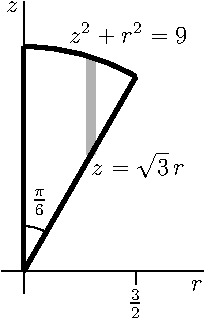
\includegraphics{fig/OE04Q8.pdf}
\end{center}


(b) In spherical coordinates, the density of is 
$\de=x^2+y^2=\rho^2\sin^2\varphi$,
the bottom of the solid is at 
\begin{equation*}
z=\sqrt{3}\,r\iff \rho\cos\varphi=\sqrt{3}\,\rho\sin\varphi\iff
\tan\varphi=\frac{1}{\sqrt{3}}\iff\varphi=\frac{\pi}{6}
\end{equation*} 
and the top of the solid is at $x^2+y^2+z^2=\rho^2=9$. 
The mass is
\begin{equation*}
m=\int_0^{2\pi}\dee{\theta}\int_0^{\pi/6}\dee{\varphi}\int_0^3\dee{\rho}\ \big(\rho^2\sin\varphi\big)
\overbrace{\big(\rho^2\sin^2\varphi\big)}^{\de}
\end{equation*}



(c) \emph{Solution 1:}\ \ \  Making the change of variables $s=\cos\varphi$, 
$\dee{s}=-\sin\varphi\ \dee{\varphi}$, in the integral of part (b),
\begin{align*}
m&=\int_0^{2\pi}\dee{\theta}\int_0^{\pi/6}\dee{\varphi}
  \int_0^3\dee{\rho}\ \rho^4\sin\varphi \big(1-\cos^2\varphi\big) \\
&=\frac{3^5}{5}\int_0^{2\pi}\dee{\theta}\int_0^{\pi/6}\dee{\varphi}\ \sin\varphi
\big(1-\cos^2\varphi\big) \\
&=-\frac{3^5}{5}\int_0^{2\pi}\dee{\theta}\int_1^{\sqrt{3}/2}\dee{s}\  (1-s^2) \\
&=-\frac{3^5}{5}\int_0^{2\pi}\dee{\theta}\ \left[s-\frac{s^3}{3}\right]_1^{\sqrt{3}/2} \\
&=2\pi \frac{3^5}{5} \left[1-\frac{1}{3}-\frac{\sqrt{3}}{2}+\frac{\sqrt{3}}{8}\right] \\
&=2\pi \frac{3^5}{5} \left[\frac{2}{3}-\frac{3\sqrt{3}}{8}\right]
\end{align*}

(c) \emph{Solution 2:}\ \ \ 
As an alternate solution, we can also evaluate the integral of part (a).
\begin{align*}
m&=\int_0^{2\pi}\dee{\theta}\int_0^{3/2}\dee{r}\ r\int_{\sqrt{3}\,r}^{\sqrt{9-r^2}}dz\ r^2\cr
&=\int_0^{2\pi}\dee{\theta}\int_0^{3/2}\dee{r}\ r^3\big(\sqrt{9-r^2}-\sqrt{3}\,r\big)\cr
&=2\pi\int_0^{3/2}\dee{r}\ r^3\big(\sqrt{9-r^2}-\sqrt{3}\,r\big)
\end{align*}
The second term
\begin{equation*}
-2\pi\int_0^{3/2}\dee{r}\ \sqrt{3}\,r^4=-2\pi\sqrt{3}\,\frac{r^5}{5}\bigg|_0^{3/2}
=-2\pi\sqrt{3}\,\frac{3^5}{5\times  2^5}
\end{equation*}
For the first term, we substitute $s=9-r^2$, $\dee{s}=-2r\,\dee{r}$.
\begin{align*}
2\pi\int_0^{3/2}\dee{r}\ r^3\sqrt{9-r^2}
&=2\pi\int_9^{27/4}\overbrace{\frac{\dee{s}}{-2}}^{r\,\dee{r}}
        \overbrace{(9-s)}^{r^2} \sqrt{s}
=-\pi \left[6s^{3/2}-\frac{2}{5}s^{5/2}\right]_9^{27/4}\cr
&=-\pi \left[\frac{3^5\sqrt{3}}{4}-2\times 3^4
         -\frac{3^7}{2^4 5}\sqrt{3}+2\frac{3^5}{5}\right]
\end{align*}
Adding the two terms together,
\begin{align*}
m&=-2\pi\frac{3^5}{5} \frac{\sqrt{3}}{32}
   -2\pi\frac{3^5}{5} \frac{5\sqrt{3}}{8}
   +2\pi\frac{3^5}{5} \frac{5}{3}
   +2\pi\frac{3^5}{5} \frac{9\sqrt{3}}{32}
   -2\pi\frac{3^5}{5}
\\
&=2\pi\frac{3^5}{5}\left[\left(\frac{5}{3}-1\right)
-\sqrt{3}\left(\frac{1}{32}+\frac{5}{8}-\frac{9}{32}\right)\right] \\
&=2\pi \frac{3^5}{5} \left[\frac{2}{3}-\frac{3\sqrt{3}}{8}\right]
\end{align*}

\end{solution}
